\documentclass[11pt, a4paper]{article}

\makeatletter
\def\input@path{{../}}
\makeatother

\usepackage{caption}
\usepackage{subcaption}
\captionsetup{font=small, labelfont=bf}
\usepackage[T1]{fontenc}
\usepackage[utf8]{inputenc}
\usepackage[margin=2.4cm]{geometry}
\usepackage{amsmath, amssymb, amsthm}
\usepackage{booktabs}
\usepackage{array}
\usepackage{tabularx}
\usepackage{multirow}
\usepackage{hyperref}
\usepackage{xcolor}
\usepackage{enumitem}
\usepackage{titlesec}
\usepackage{graphicx}
\graphicspath{{../}}
\usepackage[authoryear,round]{natbib}
\usepackage{setspace}
\usepackage{footnote}
\usepackage{float}
\usepackage{placeins}
\usepackage{eurosym}

\hypersetup{
  colorlinks=true,
  linkcolor=blue!60!black,
  citecolor=blue!50!black,
  urlcolor=blue!70!black
}

\definecolor{terracotta}{RGB}{200, 92, 72}
\definecolor{mutedgold}{RGB}{188, 145, 38}
\definecolor{emerald}{RGB}{35, 130, 75}
\definecolor{lightemerald}{RGB}{48, 168, 130}
\definecolor{cobaltblue}{RGB}{54, 118, 172}

\setstretch{1.15}
\setlength{\bibsep}{2pt}
\titlespacing*{\section}{0pt}{1.5ex plus 0.4ex minus .2ex}{0.8ex plus .2ex}
\titlespacing*{\subsection}{0pt}{1.2ex plus 0.3ex minus .2ex}{0.6ex plus .2ex}
\titlespacing*{\subsubsection}{0pt}{1.0ex plus 0.2ex minus .2ex}{0.4ex plus .2ex}

\begin{document}

\title{\Large \textbf{Should I Save \textit{and} Should I Go? A Spatial Model of Climate Change Adaptation with Saving and Migration}\thanks{This paper is the result of my Master's thesis defended at the Paris School of Economics (extended thesis version available \href{https://lchapuisb.github.io/SavingSIAM/master_thesis.pdf}{here}). I thank Katheline Schubert and Marc Fleurbaey for their guidance and continuous support. I would also like to thank Lucas Chancel and Hélène Ollivier for valuable discussions and Adrien Bilal, Martin Breux, Camille Lemonde and Eve Samani for helpful comments. All remaining errors are my own.}}
\author{
    \textbf{Léon Chapuis}\thanks{Email: \href{mailto:leon.chapuis@ens.psl.eu}{leon.chapuis@ens.psl.eu}.}
}
\date{November 2026}
\maketitle
\thispagestyle{plain}
\begin{abstract}
\noindent
I build a Dynamic Quantitative Spatial Model featuring heterogeneous agents capable of both saving and migrating across all 51 U.S. states to examine adaptation to a spatially heterogeneous climate change. This paper contributes to an emerging literature in climate macroeconomics by providing a tractable structural framework to jointly evaluate saving and migration at the individual worker level within a dynamic spatial model. I build on an existing framework which incorporates a CARA preference structure that separates workers' migration and saving choices, ensuring tractability despite the curse of dimensionality. The main result demonstrates that climate damages induce significant spatial reallocation and precautionary saving, which smooth the drop in consumption and restrict welfare losses to 0.5\%, while altering the spatial distribution of wealth. Anticipation helps to speed the transition and limits welfare drop on the transition path. Counterfactual scenarios reveal both substitutability and complementarity between saving and migration; suppressing either of these adaptive margins amplifies welfare losses, showing the interaction between wealth accumulation and spatial mobility in adapting to climate damages.
\end{abstract}
\vspace{0.8em}
\noindent \textbf{JEL classification:} Q54, R12, R23, E21, J61 \\
\textbf{Keywords:} Climate Change, Migration, Saving, Spatial Economics, Dynamic Model
\vspace{1em}

\section{Introduction}

Climate change is already underway. Global temperatures have increased by $+1.1^\circ\text{C}$ since the pre-industrial era, and IPCC projections anticipate an additional warming of $+2.0^\circ\text{C}$ to $+4.0^\circ\text{C}$ by 2100 \citep{lee_ipcc_2023}. Therefore, rather than relying only on mitigation policies, responses to climate change increasingly take the form of adaptation and behavioural adjustments. Importantly, because climate damages are heterogeneous across regions, this need for adaptation is connected to the spatial distribution of climate shocks.

However, while wealth and capital accumulation through saving are basic elements in standard macroeconomic models since \citet{solow_contribution_1956}, their integration into spatial frameworks remains challenging. This is due to a curse of dimensionality: the state space becomes prohibitively large when tracking the joint evolution of population and capital over time and space \citep{desmet_spatial_2025}. As a result, spatial models analysing climate change adaptation, despite their rich structural features, often simplify the household behaviour and do not take into account their capacity to both save and migrate, relying instead on the assumption that all income is allocated to consumption. Yet, in reality, saving and migration are jointly determined, acting as different channels for adaptation by limiting exposure to climate damages. The objective of this paper is to develop a dynamic, quantitative spatial model that incorporates both saving and migration as adaptive mechanisms to climate change, while maintaining analytical tractability.

I build on the framework developed by \citet{dvorkin_geography_2025} (hereafter DG). This is an endowment economy with $J$ locations, representing local labour markets that differ in wages, amenities, housing costs, and the variance of individual productivity shocks. Workers are risk-averse and heterogeneous, facing both uninsurable idiosyncratic productivity shocks and idiosyncratic location preference shocks. They exhibit Constant Absolute Risk Aversion (CARA) preferences, can move across locations subject to a mobility friction, and can save a fraction of their income. The primary limitation of the CARA utility function, the absence of wealth effects, is what yields closed-form solutions for consumption and saving. This preference structure ensures the analytical separation of workers' migration and saving choices, rendering the model tractable.

I introduce three innovations to this framework. First, I incorporate transitional dynamics. In the context of climate change, understanding how workers anticipate future damages and how long it takes them to fully adapt are questions of interest, and can only be captured through the length of a transition path. Second, I introduce an exogenous climate trajectory from 2010 to 2100. Building on the county-level estimates of \citet{hsiang_estimating_2017}, I map climate damages into three channels: wages, amenities, and housing costs. Third, the original DG framework does not disentangle migration costs from amenities, jointly treating them as a residual. To isolate the effect of heterogeneous amenity changes on household behaviour and to conduct counterfactuals on migration while preserving the role of amenities, I separate migration costs from amenities by parameterizing moving costs via a two-parameter gravity structure during calibration.

The model is calibrated to the US economy at the state level for the year 2010 using external parameters from \citet{dvorkin_geography_2025}, the BEA, and the ACS alongside internal moment matching, and is then simulated from 2010 to 2500 with climate damages unfolding between 2010 and 2100. Exploiting the model's tractability, I evaluate counterfactual scenarios shutting down workers' foresight or suppressing their capacity to save or migrate. The empirical analysis yields four main sets of results.

\paragraph{(i) Anticipation and adaptation in the baseline scenario.} In the baseline specification, where workers can save, migrate, and possess perfect foresight regarding future damages, anticipation and adaptation limit the aggregate impact of climate change. A strong spatial reallocation of individuals almost offsets the decline in aggregate income; Florida, for instance, loses over 80\% of its population. The anticipation of future damages induces precautionary saving between 2010 and 2100, which smooths the decline in consumption and welfare along a 300-year transition before both revert to levels comparable to 2010. In aggregate, welfare falls by 0.5\%, constituting a lower bound relative to alternative estimates. While these aggregate macroeconomic variations are modest, they mask spatial disparities across states: accumulated wealth contracts by more than 20\% in Southeastern states, yet rises by over 10\% in Montana.

\paragraph{(ii) The role of perfect foresight.} To determine the extent to which anticipation shapes behaviour, I simulate a counterfactual in which workers are myopic regarding climate change. Without anticipation, workers do not accumulate precautionary savings between 2010 and 2100. As a result, the welfare drop in 2100 is four times larger in the myopic scenario than in the baseline. Driven by spatial frictions, the wealth distribution, and the absence of foresight, convergence to the terminal steady state requires an additional 100 years relative to the perfect-foresight baseline.

\paragraph{(iii) Shutting down migration.} To quantify the importance of spatial mobility, I construct a counterfactual where migration is suppressed by setting moving costs to infinity. Without the ability to self-insure spatially, the aggregate wealth-to-income ratio surges from 4.1 to 7.3 even in the absence of climate change, demonstrating a substitutability between saving and migration. Isolating the climate shock, the peak in the wealth-to-income ratio between 2010 and 2100 reaches $+6$\% above a trajectory without climate change, compared to $+4.5$\% in the baseline. Suppressing migration generates more negative welfare consequences, driving an aggregate decline of 1.5\%.

\paragraph{(iv) Shutting down saving.} Finally, when workers are not allowed to save, allocating all income to consumption, the inter-state migration rate increases from 2.5\% to 2.7\%. This confirms the substitutability between saving and migration, in the spirit of the 'location as an asset' framework of \citet{bilal_location_2021}. Nevertheless, the absence of saving has more severe welfare implications, yielding a 2.8\% decline in long-run welfare.

Together, these scenarios show a relationship between mobility and wealth accumulation of both substitutability and complementarity, operating across time horizons and in both spatial directions, even though CARA preferences make individual migration and saving decisions independent of current wealth. Along the transition path, the two margins adjust at different speeds: liquid precautionary saving responds immediately to anticipated damages and limits medium-run welfare losses (so that anticipating damages without moving outperforms moving myopically by 2100), whereas spatial reallocation happens gradually over centuries due to moving frictions. Across space, complementarity runs both ways. First, wealth allows more effective spatial adaptation; without saving to absorb the high uninsurable variance penalty of productive Northern destinations, climate migrants are forced into sub-optimal, lower-variance regions, degrading the directional efficiency of mobility. Second, the spatial network shapes wealth accumulation; the option to migrate, combined with idiosyncratic location preferences, generates a demand for spatially heterogeneous precautionary saving.


\paragraph{Related literature.} This paper relates to three strands of literature on dynamic adaptation across space and time. First, existing work has largely examined saving and migration one adaptation margin at a time. On the saving and capital side, regional climate models following \citet{nordhaus_regional_1996} and high-resolution frameworks such as \citet{krusell_climate_2022} incorporate capital accumulation while prohibiting migration, and \citet{fried_seawalls_2022} finds that protective capital investments substantially reduce U.S.\ climate welfare costs despite small aggregate effects. On the mobility side, dynamic spatial models incorporate migration while abstracting from individual worker saving due to the high dimensionality of joint wealth and population distributions \citep{desmet_spatial_2025}. Early spatial models collapse dynamic location choices into static problems \citep{desmet_geography_2018}, as applied to global warming by \citet{cruz_economic_2024} and \citet{desmet_climate_2024}. Forward-looking migration with preference shocks and moving costs was introduced by \citet{caliendo_trade_2019} and extended to cash moving costs and climate inequality with hand-to-mouth workers by \citet{tuting_climate_2025}, while \citet{kleinman_dynamic_2023} and \citet{bilal_anticipating_nodate} separate mobile hand-to-mouth workers from immobile capitalists.

A second, recent strand combines endogenous worker wealth with geographic mobility, mostly outside climate applications and restricted to steady states or small shocks: \citet{giannone_unpacking_2023} use an overlapping generations framework, \citet{donald_optimal_2025} apply a sequence-space Jacobian under small aggregate shocks, \citet{greaney_dynamic_2025} use mixed continuous-discrete time, and \citet{dvorkin_geography_2025} obtain closed-form steady-state rules under CARA preferences. Conceptually, this work builds on whether saving and migration act as substitutes (self-insurance versus self-protection in \citet{ehrlich_market_1972}, or ``location as an asset'' in \citet{bilal_location_2021}), or as complements, as in target-saving migration models \citep{berninghaus_role_1993}.

Third, two recent papers bring joint saving and migration to climate change via intensive numerical methods: \citet{abajian_savings_2025} models global borrowing-constraint liquidity traps, and \citet{sun_wealth_2025} studies U.S.\ housing wealth using deep learning. Both capture rich financial or housing frictions, at the cost of some black-box dynamics. This paper makes the opposite methodological trade-off: extending the CARA tractability of \citet{dvorkin_geography_2025} to 500-year climate transitions, while separating bilateral moving costs from time-varying amenities, trades borrowing constraints and endogenous housing prices for closed-form policy rules that trace and decompose each saving and spatial mechanism.

The rest of the paper is organised as follows. Section~\ref{sec:model} presents the dynamic spatial model of migration and saving under uninsurable labour-income and preference shocks, together with the transition-path algorithm. Section~\ref{sec:calibration} brings the model to the data and maps empirical climate damages into wages, amenities, and housing costs. Section~\ref{sec:baseline} presents the baseline perfect-foresight climate transition at the aggregate and state levels. Section~\ref{sec:mechanisms} derives the analytical saving motives and decomposes steady-state wealth shifts across space. Section~\ref{sec:counterfactuals} evaluates counterfactuals on expectations, mobility, and saving, and compares welfare outcomes across scenarios. Section~\ref{sec:discussion} discusses the main assumptions and concludes.


\section{Model}
\label{sec:model}
In this section, building on \citet{dvorkin_geography_2025}, I show how I introduce spatially heterogeneous climate change damages and a dynamic transition path into a spatial economy where workers can both save and migrate.\footnote{The static worker problem follows section 3 of \citet{dvorkin_geography_2025}; see their paper for details.} This is an endowment economy without production with exogenous wages, prices and interest rates. Savings are thus not transformed into capital, do not affect the interest rate, and serve solely as the workers' accumulated wealth. Time is discrete and each period represents one year.\footnote{Details for the resolution and algorithms can be found in Appendix~\ref{app:proofs} and \ref{app:algorithms}.}

\subsection{Core Structure and Assumptions}
\paragraph{The Spatial Economy.} The economy consists of $J$ locations, each representing a local labour market. Each location $j$ is characterised by a set of state-specific fundamentals that can vary over time, the wage $w_{j,t}$, the amenity $A_{j,t}$, and the housing cost $q_{j,t}$. The space is populated by a continuum of workers of measure one, each facing at each period a probability of death $\delta$ (Blanchard-Yaari perpetual youth). At each period a cohort of measure $\delta$ is born. 

Individuals have the option to move to a different labour market at the beginning of each period. I capture moving frictions with parameter $\psi_{j,\ell}$, which scales utility due to non-pecuniary costs of relocating from labour market $j$ to $\ell$, with  $\psi_{j,j} = 0$, and  $\psi_{j,\ell} \geq 0$, for $j \neq \ell$. In addition, mobility and reallocation decisions are influenced by idiosyncratic preference shocks for different labour markets. These shocks are denoted by the random vector $\varepsilon \in \mathbb{R}^J_+$, where each element is distributed i.i.d. Weibull with shape parameter $\nu \geq 0$ and identical scale parameter $\lambda = \bar{\lambda}\frac{J^{-1/\nu}}{\Gamma(1+\nu)}$. $\nu$ is proportional to the inverse of the variance of $\varepsilon$.

The scale parameter $\lambda$ is chosen such that the expected value of the maximum of $J$ i.i.d. Weibull random variables is $\bar{\lambda}$, ensuring that the average idiosyncratic preference shock across locations is consistent with the model's calibration. Beyond governing mobility, these uninsurable preference shocks introduce an additional source of risk. For instance, workers residing in high-wage locations face the risk of drawing a strong preference shock for a lower-wage region. Because satisfying this preference forces a geographic transition that will reduce their future disposable income, these preference shocks generate a spatial precautionary savings motive.

\paragraph{Income Process and Incomplete Markets.} The total efficient units of labour supplied inelastically by worker $i$ are $(1 + z'_i + \eta'_i)$. $z'_i$ is an AR(1) process with shock $\epsilon'_i$ so $z'_i = \rho z_i + \epsilon'_i$. $\epsilon'_i$ and $\eta'_i$ are i.i.d. shocks distributed normally with mean zero and variance $\sigma^2_{\epsilon, \ell}$ and $\sigma^2_{\eta, \ell}$, respectively. The autocorrelation parameter $\rho \in [0,1]$ is common across all labour markets, but the variances of the shocks can differ across regions. $z'_i$ is the persistent income shock and $\eta'_i$ the transitory income shock. To solve the model numerically, this continuous stochastic process is discretised into $N_z = 15$ grid nodes using the Rouwenhorst method.\footnote{With a slight abuse of notation, I occasionally write sums over $z$ in place of integrals when referring to the discretised state space or numerical moments.}

Workers have no access to state-contingent claims to insure against the individual labour income fluctuations and the idiosyncratic preference shocks. Workers have access to a global financial market where they can partially hedge against shocks by borrowing or saving in a risk-free bond. Bonds can be purchased at the price of $1/(1 + r_t)$ units of final consumption at date $t$ and each bond pays one unit of the final consumption good the next period if the bondholder survives. Newborn workers start with an exogenous and identical level of assets $a_0$ and $z = 0$.

\paragraph{Climate Change.} The economy is hit by an exogenous climate change shock that affects the fundamentals of each location. The climate change shock is represented by a vector of three components: $D^w_{j,t}$, $D^A_{j,t}$, and $D^q_{j,t}$, which represent the changes in wages, amenities, and housing costs in location $j$ at time $t$, respectively. The wage and housing shocks ($D^w_{j,t}$, $D^q_{j,t}$) enter multiplicatively as proportional changes, whereas the amenity shock ($D^A_{j,t}$) enters additively in utility units. The shocks are assumed to be exogenous and permanent. The climate change shocks are assumed to be known by the workers, and they can anticipate the future path of these shocks when making their saving and migration decisions.

\paragraph{The Workers.} The utility function exhibits Constant Absolute Risk Aversion (CARA), with the parameter $\gamma$ representing the coefficient of absolute risk aversion. The intra-period utility of a worker residing in location $j$ at time $t$ depends on the level of consumption $c$ and the amenity $A$ enjoyed and is given by:
\begin{equation}
u(c_{j,t}(a, z^\prime, \eta^\prime), A_{j,t}) = -\frac{1}{\gamma} e^{-\gamma c_{j,t}(a, z^\prime, \eta^\prime) - (A_{j,t} - D^A_{j,t})}
\end{equation}
Importantly, markets are incomplete but workers face no borrowing constraints, allowing them to save or borrow any amount they choose.\footnote{The transversality condition is naturally imposed for the value function to be well-defined: $\lim_{t \rightarrow +\infty}\frac{a_{j,t}}{(1 + r_t)^t} = 0$.} Conditional on having chosen destination $j$, their budget constraint is given by:
\begin{equation}
c_{j,t}(a, z^\prime, \eta^\prime) + \frac{a_{j,t+1}}{1 + r_t} + q_{j,t}(1+ D^q_{j,t}) = w_{j,t}(1-D^w_{j,t})(1 + z^\prime + \eta^\prime) + a
\label{eq:budget}
\end{equation}
The timing of the model is as follows: 
\begin{enumerate}[noitemsep, topsep=2pt]
  \item Entering the period with asset holdings $a$, past persistent productivity $z$, and an origin location, workers draw their idiosyncratic location preference shocks $\varepsilon$ and observe the climate-adjusted fundamentals of all locations ($w$, $A$, and $q$).
  \item Based on their state variables and the observed fundamentals, they choose their destination location $j$.
  \item After relocating, they draw their new idiosyncratic income shocks: the persistent component $z^\prime$ and the transitory component $\eta^\prime$.
  \item Based on the realisation of the income shocks, they choose their consumption $c_{j,t}$ and next-period savings $a_{j,t+1}$.
  \item Between periods, workers face a probability of death $\delta$ and are replaced by newborns with initial asset holdings $a_0$ and $z = 0$.
\end{enumerate}

\subsection{Workers' Program}
\label{sec:workers_program}
Let $V_{j,t}(a, z, \varepsilon)$ be the ex-ante value function of a worker starting the period in origin location $j$. Because of the CARA utility formulation, the moving friction $e^{\psi_{j\ell}}$ and the preference shock $\varepsilon_\ell$ act as multiplicative scalars on the exponential utility and cancel out of the intra-period first-order conditions. It makes the optimal consumption and saving choices depend only on the chosen destination $\ell$ and the idiosyncratic states, remaining independent of the origin $j$. The worker's problem is defined as:
\begin{equation}
V_{j,t}(a, z, \varepsilon) = \max_{\ell} \left\{ \varepsilon_\ell e^{\psi_{j\ell}} \mathbb{E}_{\eta^\prime, z^\prime | z, \ell} \left[ \max_{c_{\ell,t}, a_{\ell,t+1}} \left\{ -\frac{1}{\gamma} e^{-\gamma c_{\ell,t} - (A_{\ell,t} - D^A_{\ell,t})} + \beta \mathbb{E}_{\varepsilon^\prime} \left[ V_{\ell,t+1}(a_{\ell,t+1}, z^\prime, \varepsilon^\prime) \right] \right\} \right] \right\}
\end{equation}
subject to the conditional budget constraint in destination $\ell$ given by Equation~\eqref{eq:budget}.

\paragraph{Program's Solution.} Due to the CARA utility specification, the Weibull distribution of preference shocks, and the absence of borrowing constraints, the worker's problem can be solved in closed form.\footnote{This is Proposition 1 of \citet{dvorkin_geography_2025} with a slight simplification.} For the sake of clarity let $\tilde{y}_{\ell,t} = (1 - D^w_{\ell,t})w_{\ell,t} - q_{\ell,t}(1+ D^q_{\ell,t})$,  $\tilde{w}_{\ell,t} = (1 - D^w_{\ell,t})w_{\ell,t}$ and $\tilde{A}_{\ell,t} = A_{\ell,t} - D^A_{\ell,t}$. In addition, denote the \textit{ex ante} lifetime utility function as $v_{j,t}(a, z) = \mathbb{E}_\varepsilon\left(V_{j,t}(a, z, \varepsilon)\right)$. Under a stationary interest rate $r_t = r$, the marginal propensity to consume out of wealth is constant and equal to $\frac{r}{1+r}$. The optimal consumption-savings decisions of a worker, after having chosen destination location $\ell$, are characterised by:
\begin{align}
c_{\ell,t}(a, z^\prime, \eta^\prime) &= \Xi_{\ell,t}(z^\prime) + \frac{r}{1+r} \left[ \tilde{y}_{\ell,t} + \tilde{w}_{\ell,t}\eta^\prime + a \right] \label{eq:cpol} \\
a_{\ell,t+1}(a, z^\prime, \eta^\prime) &= \left[ \tilde{y}_{\ell,t} + \tilde{w}_{\ell,t}\eta^\prime + a \right] + (1+r) \left( \tilde{w}_{\ell,t}z^\prime - \Xi_{\ell,t}(z^\prime) \right) \label{eq:apol}
\end{align}
where $\Xi_{\ell,t}(z^\prime)$ depends on the realisation of the persistent shock $z^\prime$, the selected labour market, and time. Moreover, the share of individuals moving from labour market $j$ to $\ell$, $\mu_{j\ell,t}(z)$, are given by:
\begin{equation}
\mu_{j\ell,t}(z) = \frac{ e^{\nu \mathbb{B}_{1,j\ell,t}} \left( \mathbb{E}_{z^\prime | z, \ell} \left[ e^{-\gamma \Xi_{\ell,t}(z^\prime)} \right] \right)^{-\nu} }{ \sum_{m=1}^J e^{\nu \mathbb{B}_{1,jm,t}} \left( \mathbb{E}_{z^\prime | z, m} \left[ e^{-\gamma \Xi_{m,t}(z^\prime)} \right] \right)^{-\nu} }
\label{eq:mu}
\end{equation}
where the location-to-destination specific value shifter is defined as $\mathbb{B}_{1,j\ell,t} = \tilde{A}_{\ell,t} - \psi_{j\ell} + \gamma \left(\frac{r}{1+r}\right) \tilde{y}_{\ell,t} - \frac{1}{2}\left(\frac{r}{1+r} \gamma \tilde{w}_{\ell,t}\right)^2 \sigma_{\eta,\ell}^2$. The continuation term $\Xi_{\ell,t}(z^\prime)$ is defined recursively as:
\begin{align}
\Xi_{\ell,t}(z^\prime) &= -\frac{1}{\gamma(1+r)} \Bigg( \log(\beta(1+r)) - \gamma r \tilde{w}_{\ell,t}z^\prime + \tilde{A}_{\ell,t} + \log(\bar{\lambda}) \nonumber \\
&\quad - \frac{1}{\nu} \log \left[ \frac{1}{J} \sum_{m=1}^J e^{\nu \mathbb{B}_{1,\ell m, t+1}} \left( \mathbb{E}_{z^{\prime\prime} | z^\prime, m} \left[ e^{-\gamma \Xi_{m,t+1}(z^{\prime\prime})} \right] \right)^{-\nu} \right] \Bigg) \label{eq:Xi}
\end{align}
Economically, the endogenous term $\Xi_{\ell,t}(z^\prime)$ acts as a state-dependent intercept in the consumption rule. It captures all forward-looking components of the household's problem, including the present value of expected future permanent income, the precautionary savings motive against spatial and income risks, and the option value of future geographic mobility. It is important to note that $\Xi_{\ell,t}(z^\prime)$ is independent of $a$: the state space reduces from $(a, z, \ell)$ to $(z, \ell)$ and the model is thus tractable, making the migration decision independent of the saving decision. 

Another interesting property of this economy is the spatial sorting of high productivity workers (the ones with a high $z$) in high wage locations. As the gain from a high $z$ is multiplied by the local wage, highly productive workers benefit more from high-wage locations and as $z$ is persistent, the chance of moving to a high wage location is higher for high-$z$ workers than low-$z$ workers. At the aggregate level, let $\Lambda_t(\ell, z)$ denote the density of workers with persistent productivity $z$ residing in location $\ell$ at period $t$ (normalised to unit national mass, $\sum_{\ell=1}^J \int \Lambda_t(\ell, z)\,\mathrm{d}z = 1$), $L_{\ell,t} = \int \Lambda_t(\ell, z)\,\mathrm{d}z$ the local population share of state $\ell$, and $\bar{a}_t(\ell, z)$ the mean asset holdings in $(\ell, z)$. Their laws of motion and aggregation formulas are detailed in Appendix~\ref{app:proofs}.\footnote{This is Proposition 2 of \citet{dvorkin_geography_2025}.}

\subsection{Computation of the Dynamic Transition}
\label{sec:transition}

Because the original paper compares only two steady states, I introduce a transition-path algorithm. A key property of the CARA specification is that the value-function index $\Xi_\ell(z)$ does not depend on asset holdings~$a$ (cf.\ Subsection~\ref{sec:workers_program}). This implies that migration probabilities $\mu_{j\ell}(z)$ are also independent of~$a$, which yields a three-stage decomposition: the value function, the population distribution, and the wealth distribution can each be solved sequentially, without joint iteration.
\begin{equation}
  \underbrace{\Xi_T \to \Xi_{T-1} \to \cdots \to \Xi_1}_{\text{Backward: no $\Lambda$, no $a$}}
  \quad\longrightarrow\quad
  \underbrace{\Lambda_0 \to \Lambda_1 \to \cdots \to \Lambda_T}_{\text{Forward: no $a$}}
  \quad\longrightarrow\quad
  \underbrace{\bar a_0 \to \bar a_1 \to \cdots \to \bar a_T}_{\text{Forward: uses both}}
  \label{eq:three_stage}
\end{equation}

\paragraph{Parameter paths.} Climate change damages are phased in linearly between the initial and terminal steady states: for each time-varying sequence $x \in \{w,\, \tilde w,\, \tilde y,\, \sigma^2_\epsilon,\, \sigma^2_\eta,\, A,\, q\}$, a linear ramp $x_\ell(t) = x_{\ell,0}(1 - t/T_{\text{shock}}) + x_{\ell,T_{\text{shock}}}(t/T_{\text{shock}})$ is constructed over the damage horizon $t = 0,\ldots,T_{\text{shock}}$, and held constant at its terminal post-damage value for $t > T_{\text{shock}}$ up to $T_{\text{sim}} = 500$.

\paragraph{Stage 1: Backward induction on $\Xi$.}
The terminal condition is $\Xi_T = \Xi^*_{SS,T}$, the fixed point of eq.~\eqref{eq:Xi} under the terminal post-damage parameters. The algorithm sweeps backward from $t = T{-}1$ to $t = 1$: at each date $t$, evaluating the climate-adjusted wages, amenities, and housing costs at $t$ and $t{+}1$ along their linear ramp (together with the income transition matrices $\{\Pi^\ell_{t+1}\}_\ell$), a single application of eq.~\eqref{eq:Xi} yields $\Xi_t$ from $\Xi_{t+1}$.

\paragraph{Stage 2: Forward simulation of $\Lambda$.}
Starting from $\Lambda_0 = \Lambda^*_{SS,0}$, the population distribution is propagated forward as a matrix product. At each $t$, the migration probability array $\mu_{j\ell}(z)$ is computed from $\Xi_t$ and $\mathbb{B}_{1,j\ell,t}$. A  $(JN_z)\times(JN_z)$ transition matrix $\mathbf{T}_t$ is then assembled, with entries:
\begin{equation}
  T_t\bigl((j,z),\,(\ell,z')\bigr)
  = (1-\delta)\,\mu_{j\ell}(z)\,\Pi^\ell_{z,z'}
  \;+\;\delta\,\mu_{j\ell}(z{=}0)\,\Pi^\ell_{0,z'},
  \label{eq:T_sparse}
\end{equation}
where the first term governs surviving agents and the second governs newborns replacing the dead (born at $z=0$, allocated using the same migration probabilities evaluated at the median grid point). The forward update reduces to $\boldsymbol{\Lambda}_{t+1} = \boldsymbol{\Lambda}_t \cdot \mathbf{T}_t$ ($\boldsymbol{\Lambda}_t \in \mathbb{R}^{1 \times JN_z}$), followed by renormalisation to unit mass.

\paragraph{Stage 3: Forward computation of wealth.}
Per-capita wealth $\bar a_t(\ell,z)$ is updated forward from the initial condition $\bar a_0 = \bar a^*_{SS,0}$. Because the CARA savings rule (eq.~\ref{eq:apol}) is affine in~$a$, mean wealth evolves linearly. Decomposing the wealth mass arriving at state $(\ell, z')$ into three components:
\begin{equation}
  \underbrace{\sum_{j,z}\Lambda_t(j,z)\,\bar a_t(j,z)\,T^{\mathrm{surv}}_{(j,z),(\ell,z')}}_{\text{survivor wealth transfer}}
  +\;\underbrace{\Lambda_{t+1}(\ell,z')\cdot S_\ell(z')}_{\text{income at destination}}
  +\;\underbrace{\text{NB}_{(\ell,z')}\cdot a_0}_{\text{newborn endowment}},
  \label{eq:a_bar_update}
\end{equation}
where $S_\ell(z') = \tilde y_\ell + (1{+}r)[\tilde w_\ell z' - \Xi_\ell(z')]$ is the net savings increment for an agent arriving at $(\ell,z')$ with zero initial wealth, and $T^{\mathrm{surv}}$ is the survivor-only transition matrix (first term of eq.~\ref{eq:T_sparse}). The survivor wealth transfer is again a single matrix--vector product; per-capita wealth is then recovered by dividing by $\Lambda_{t+1}$.


\section{Calibration}
\label{sec:calibration}
This section explains how the model is brought to the data. Table~\ref{tab:baseline_params} reports parameter values that are common across states.

\begin{table}[!htb]
    \centering
    \small
    \caption{Baseline Global Parameters}
    \label{tab:baseline_params}
    \begin{tabular}{llcc}
        \toprule
        \textbf{Description} & \textbf{Parameter} & \textbf{Value} & \textbf{Calibration} \\
        \midrule
        \multicolumn{4}{l}{\textbf{\textit{Preferences \& Demographics}}} \\
        Discount factor & $\beta$ & $0.971$ & External \\
        Absolute risk aversion (CARA) & $\gamma$ & $3.000$ & External \\
        Per-period death rate & $\delta$ & $0.025$ & External \\
        Newborn wealth & $a_0$ & $0.000$ & External \\
        Migration elasticity (Weibull shape) & $\nu$ & $3.950$ & External \\
        Preference shock scale parameter & $\bar{\lambda}$ & $0.371$ & Internal \\
        \midrule
        \multicolumn{4}{l}{\textbf{\textit{Income Process}}} \\
        Autocorrelation of persistent shock & $\rho$ & $0.934$ & External \\
        Shock variances & $\sigma_{\epsilon,\ell}^2$, $\sigma_{\eta,\ell}^2$ & 51 states (DG, 2025) & External \\
        \midrule
        \multicolumn{4}{l}{\textbf{\textit{Spatial Economy \& Migration Costs}}} \\
        Interest rate & $r$ & $0.030$ & External \\
        Fixed migration cost & $\psi_{\text{fix}}$ & $1.633$ & Internal \\
        Distance elasticity & $\psi_{\text{dist}}$ & $0.405$ & Internal \\
        Local amenities & $A_\ell$ & 51 states (inner loop) & Internal \\
        Local base wages & $w_\ell$ & 51 states (DG, 2025) & External \\
        \bottomrule
    \end{tabular}
\end{table}
\subsection{External Calibration}
The interest rate is set at $r_t = r = 0.03$ and the discount factor to $\beta = 1/(1+r) = 0.971$. $\gamma$, which captures both absolute risk aversion and prudence is set at 3, lying at the midpoint of the existing literature. The housing costs $q_{\ell, t}$ are denoted: $q_{\ell, t} = \alpha_h \frac{RPP_\ell}{100}$. $\alpha_h$ is the housing-to-income ratio at the national scale that I weight with the relative price of housing across states. $\alpha_h$ is set to 0.3 using data from the Bureau of Labour Statistics and I use the data from the Bureau of Economic Analysis for the year 2010-2015 for the relative price of housing. For simplicity, those values are fixed over time.
\paragraph{Income process.} To parameterise the spatialised income process, I adopt the estimates from \citet{dvorkin_geography_2025}. Their calibration strategy relies on a simulated method of moments that corrects for the dynamic selection of workers across space. They estimate state-level base wages ($w_\ell$), persistent shock variances ($\sigma_{\epsilon,\ell}^2$), and transitory shock variances ($\sigma_{\eta,\ell}^2$) by matching moments of residual log-earnings from the CPS-ORG (2010--2019) for employees who do not move, while using migration flows from the IRS SOI (2015--2016) to account for endogenous selection. Finally, the autoregressive parameter of the persistent shock ($\rho$) is assumed to be spatially homogenous and is calibrated to match the ratio of second-to-first-order autocovariances using panel data from the PSID (1991--1997).

\subsection{Internal Calibration}

\paragraph{Parameters specification.} To govern spatial frictions, bilateral migration costs are parameterised using a gravity-style specification: \begin{equation}
  \psi_{j\ell} = \psi_{\text{fix}} + \psi_{\text{dist}} \log(\text{dist}_{j\ell} + 1).
\end{equation}

Unlike models that use non-parametric $J \times J$ moving cost matrices \citep[e.g.,][]{dvorkin_geography_2025}, imposing this specification breaks the collinearity between bilateral frictions and location-specific amenities. This choice allows the model to identify baseline amenities $A_\ell$ from population shares (conditional on the specification not being biased), which is necessary for implementing climate damage shocks to amenities ($D^A$). However, this restriction introduces an identification challenge regarding the migration parameters ($\psi$) and the migration elasticity (the Weibull shape parameter, $\nu$). Because multiple pairs of $(\psi, \nu)$ can match the static aggregate moments while yielding different dynamic responses to shocks, these parameters cannot be identified together.\footnote{This is mentioned by \citet{sun_wealth_2025}, where $\psi_{\text{fix}}$ is externally calibrated and $\nu$ is internally calibrated.}

To resolve this, I set the migration elasticity to $\nu = 3.95$, aligning with \citet{dvorkin_geography_2025} and the broader dynamic spatial literature \citet{caliendo_trade_2019, kleinman_dynamic_2023, kennan_effect_2011}.  Because my moving cost specification is relatively smooth, it cannot capture the asymmetry of state-to-state migration flows. If $\nu$ were to be calibrated internally, the solver would be forced to generate a lower value, injecting random noise into worker location decisions to compensate for the rigid and smooth moving costs and fit the data.

\paragraph{Algorithm.}
The calibration routine employs a nested fixed-point procedure. The outer loop uses a numerical solver to calibrate the vector of aggregate parameters $\theta = (\psi_{\text{fix}}, \psi_{\text{dist}}, \bar\lambda)$ to match three targeted aggregate moments: the overall interstate migration rate, the average log-distance of moves, and the aggregate wealth-to-earnings ratio. In addition, for each guess of $\theta$, an inner loop applies a contraction mapping to iteratively update the amenity vector $\{A_\ell\}$ until the model-generated population shares match empirical population distributions. 

\paragraph{Calibration routine results.} The contraction mapping produces an amenity vector $\{A_\ell\}$ with cross-sectional mean zero (by normalisation). The distribution is economically sensible: large, high-wage states attract a compensating positive amenity value (California: $A = 0.902$; New York: $A = 0.609$; Texas: $A = 0.557$), while sparsely populated states receive negative values. All targeted moments (the three aggregate moments and the state population shares) are matched to high precision (see Table~\ref{tab:calibration_fit}).

\begin{table}[!htb]
\centering
\small
\caption{Targeted Aggregate Moments and Model Fit}
\label{tab:calibration_fit}
\begin{tabular}{lrr}
\toprule
Moment & Target & Model \\
\midrule
Aggregate out-migration rate & 0.0250 & 0.0250 \\
Aggregate wealth-to-earnings ratio & 4.0900 & 4.0888 \\
Max.\ abs.\ error in population shares & $<10^{-5}$ & $5.8 \times 10^{-7}$ \\
Average log-distance of moves & 0.5032 & 0.5032 \\ 
\bottomrule
\end{tabular}
\end{table}

Under this calibration, the model over-predicts the micro-level spatial sorting of productivity relative to the data, yielding a model-implied spatial sorting slope (the regression coefficient of $\mathbb{E}(z|j)$ on $\log(w_j)$) of approximately $0.20$, compared to the empirical benchmark of $0.11$ of \citet{dvorkin_geography_2025}. I accept this trade-off to prioritise the macro migration elasticity. As a robustness check, I evaluate a specification where $\nu$ is calibrated internally alongside the moving costs: the internal solver drives the elasticity down to $\nu = 2.18$ to fit the spatial sorting data, predicting less migration response to climate change, though the qualitative conclusions of the paper remain unchanged (results available upon request).

\paragraph{Out-of-sample fit.} The model generates a per-state value of wealth that can be compared to empirical wealth data. The model fits the data well, with a strong positive correlation between the model-generated and empirical wealth values across states (See Figure \ref{fig:out_sample_fit}).\footnote{I use the Geowealth Data from \cite{suss_geowealth-us_2024} to compare with the model-generated values with empirical data. \cite{dvorkin_geography_2025} use the individual-level data of the SIPP survey to construct the empirical data. They show that the two datasets are similar.} Furthermore, despite the restricted two-parameter gravity specification (fixed cost and distance), the model remains capable of capturing the U.S. interstate mobility out-of-sample. While the calibration routine only targets aggregate spatial frictions, the model successfully predicts the micro-level distribution of bilateral flows across all 2,550 possible state-to-state combinations. The predicted matrix exhibits a strong Pearson correlation of $0.7214$ with the empirical interstate flow matrix.

\begin{figure}[!htp]
    \centering
    \caption{Out-of-sample fit of the model}
    \label{fig:out_sample_fit}
    \begin{subfigure}[b]{0.32\textwidth}
        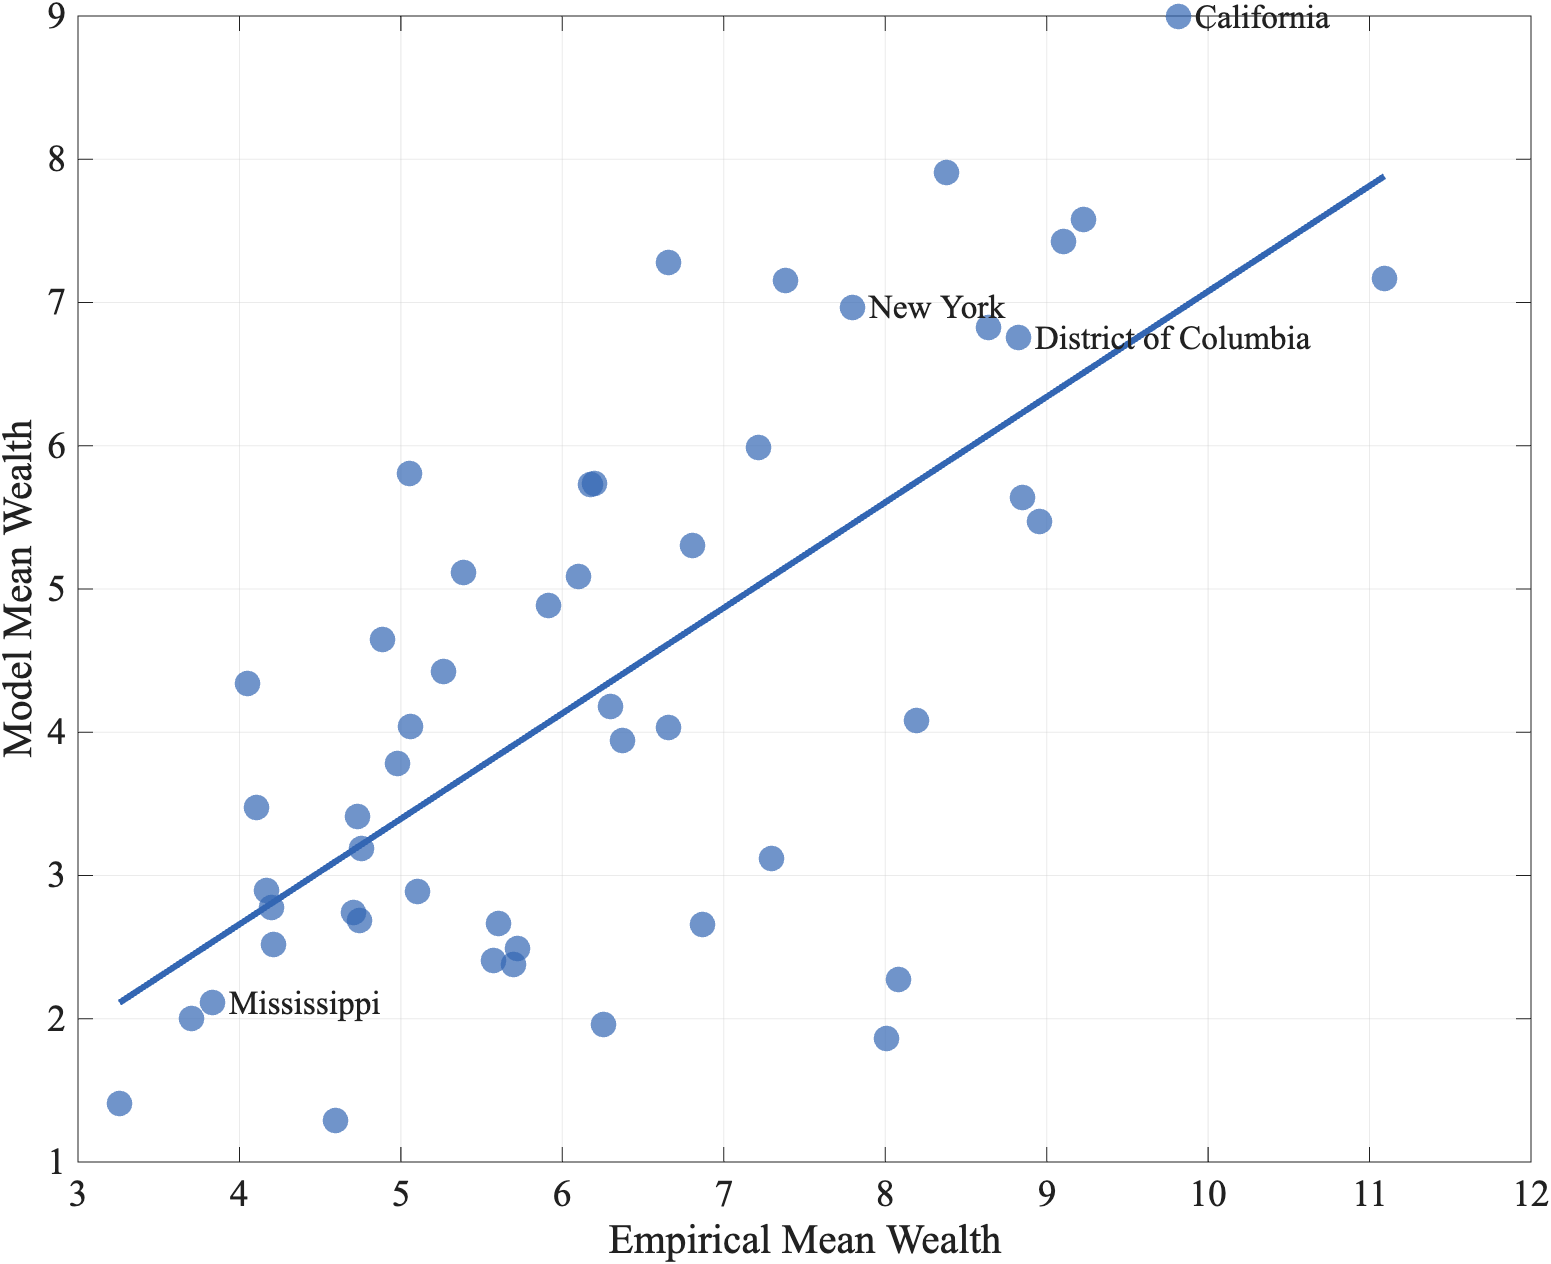
\includegraphics[width=\textwidth]{../Output/graph_comparison/out_sample_fit/out_sample_fit_model_mean_wealth.png}
        \caption{Wealth Comparisons}
        \label{fig:out_sample_wealth}
    \end{subfigure}\hfill
    \begin{subfigure}[b]{0.32\textwidth}
        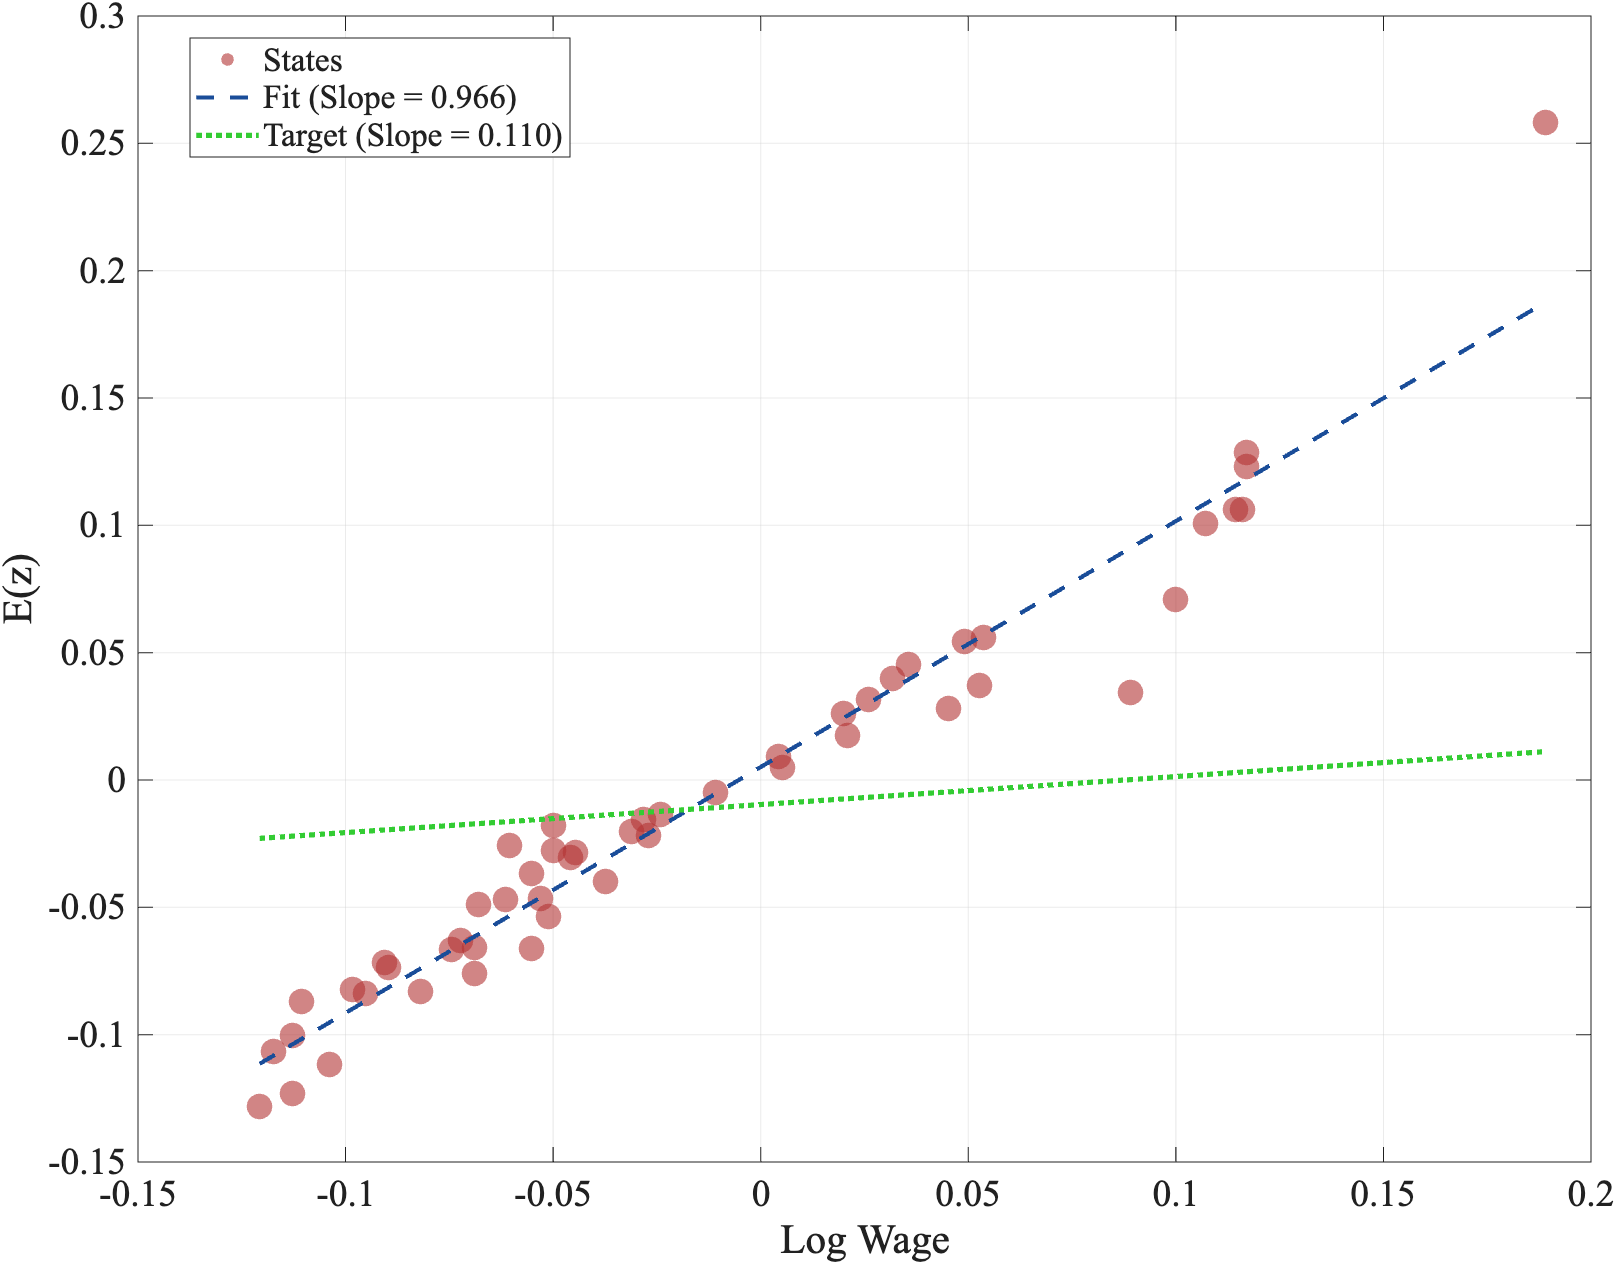
\includegraphics[width=\textwidth]{../Output/graph_comparison/out_sample_fit/out_sample_fit_e_z.png}
        \caption{Migration Sorting}
        \label{fig:out_sample_sorting}
    \end{subfigure}\hfill
    \begin{subfigure}[b]{0.32\textwidth}
        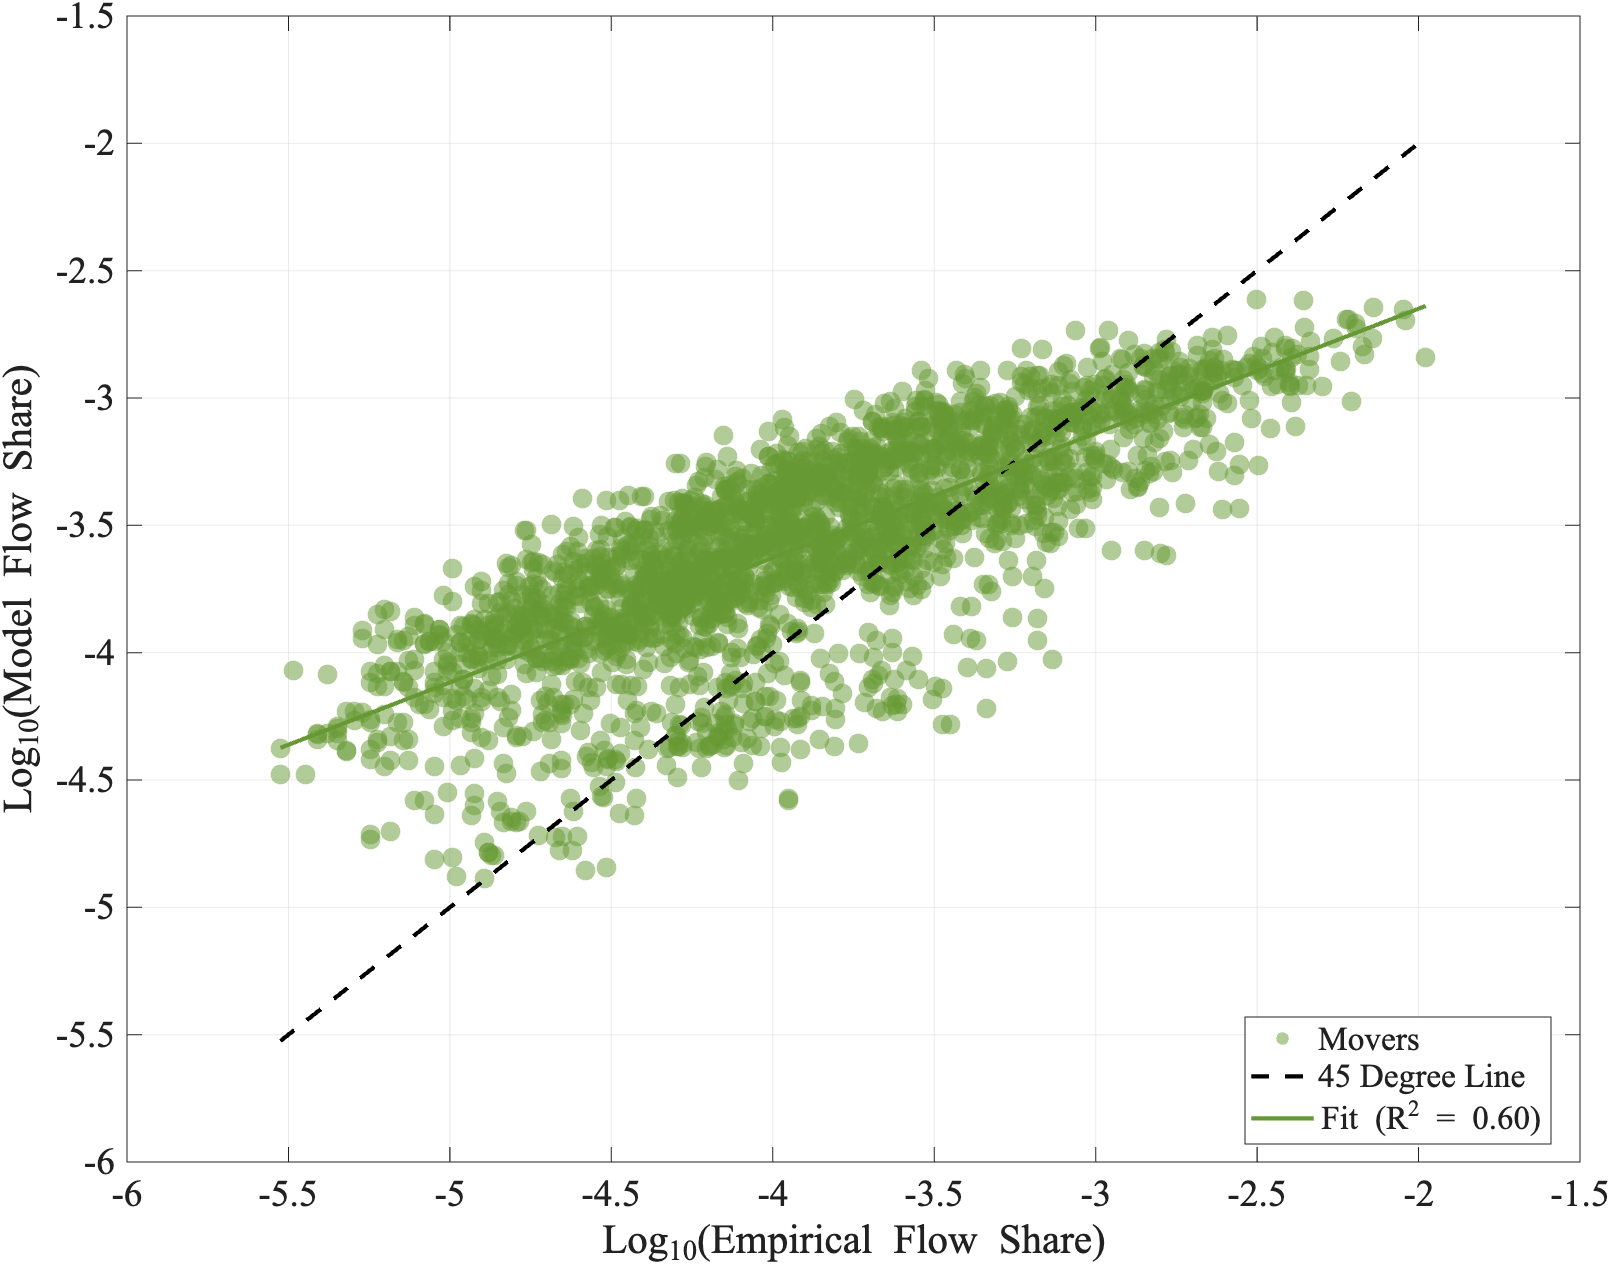
\includegraphics[width=\textwidth]{../Output/graph_comparison/out_sample_fit/out_sample_fit_log_10_model_flow_share.png}
        \caption{Bilateral Migration Flows}
        \label{fig:out_sample_flows}
    \end{subfigure}
    \begin{minipage}{\textwidth} \vspace{0.5em}
      \footnotesize{\textbf{Note:} Out-of-sample fit of the model along three dimensions: (a) average state-level wealth, (b) spatial sorting of productive workers across states, and (c) bilateral migration flows (in log shares) between states. In panel (a), the black line displays the OLS regression of model-implied mean wealth on empirical values from Geowealth-US 2010. In panel (b), the regression of expected productivity $E(z)$ on log wages (blue dashed line) is compared against the benchmark slope of $0.11$ (green dotted line) from \cite{dvorkin_geography_2025}. In panel (c), the OLS regression of model-implied bilateral log migration shares on empirical values from the ACS 2010-2019 is shown.}
    \end{minipage}
\end{figure}

\FloatBarrier
\subsection{Climate Change Damages}
The exogenous climate shock paths are derived from the county-level damage estimates of \citet{hsiang_estimating_2017}, who project economic impacts across six sectors under RCP~8.5 for the period 2080--2099. Their county-level data are aggregated to the state level using population and income weights, then mapped into the three channels of the Dvorkin \& Greaney framework (Table~\ref{tab:sector_mapping}):
\input{tables/sector_mapping.tex}
\paragraph{Sector-to-channel mapping.} Because baseline amenities ($A_{\ell, \text{init}}$) are residuals centred around zero, absolute amenity shocks ($\text{shock\_amenity}_\ell$) are interpreted as consumption-equivalent welfare losses via the marginal rate of substitution ($MRS_{A,c} = 1/\gamma$), scaling the monetary costs of mortality and crime by national average income ($\bar{Y}_{\text{US}}$). The three composite shocks are constructed as:
\begin{align}
  \text{shock\_wage}_\ell &= \frac{\bar L_\ell}{100}
    + \frac{\bar Y_\ell^{\text{agri}}}{100} \cdot s_\ell^{\text{agri}}
    - \frac{\bar C_\ell}{100}, \label{eq:shock_wage} \\
  \text{shock\_amenity}_\ell &= \gamma \left[ \left(\frac{\bar M_\ell}{100{,}000}\right) \frac{\text{VSL}}{\bar{Y}_{\text{US}}} + \left(\frac{\bar R_\ell}{100{,}000}\right) \frac{\mathbb{E}[\text{VSC}]}{\bar{Y}_{\text{US}}} \right], \label{eq:shock_amenity} \\
  \text{shock\_housing}_\ell &= \frac{\bar E_\ell}{100} \cdot s_\ell^{\text{energy}}, \label{eq:shock_housing}
\end{align}
where $\bar L_\ell$ is the income-weighted average labour productivity loss (\%), $\bar Y_\ell^{\text{agri}}$ the income-weighted agricultural yield change (\%), $s_\ell^{\text{agri}}$ the agriculture GDP share of state $\ell$ (BEA 2010--2015 average), $\bar C_\ell$ the income-weighted coastal damage (\% of county income), $\bar M_\ell$ the population-weighted additional mortality (deaths per 100k), $\bar R_\ell$ the population-weighted additional crime (crimes per 100k), $\bar E_\ell$ the income-weighted change in energy expenditures (\%), and $s_\ell^{\text{energy}}$ the state-level electricity expenditure share of personal income. For the amenity parameters, $\gamma$ is the CARA absolute risk aversion coefficient, $\text{VSL} = \$9.0\text{M}$ (2012 USD), and the expected unit cost of crime $\mathbb{E}[\text{VSC}]$ evaluates separately violent (\$205,782) and property (\$4,799) crimes following \citet{mccollister_cost_2010} and pooled with FBI UCR incident data. $\bar{Y}_{\text{US}} = \$48,668.71$ (2012 USD) is the national average income using the CPS-ORG data with the 2010--2015 average and the same restrictions as \citet{dvorkin_geography_2025}. These shocks enter the terminal steady state as $w_{\ell, \text{term}} = w_{\ell, \text{init}} \cdot (1 + \text{shock\_wage}_\ell)$, $A_{\ell, \text{term}} = A_{\ell, \text{init}} - \text{shock\_amenity}_\ell$, and $q_{\ell, \text{term}} = q_{\ell, \text{init}} \cdot (1 + \text{shock\_housing}_\ell)$.

\paragraph{Magnitudes.}
In Table~\ref{tab:shock_magnitudes}, the wage channel experiences an average decline of 1.0\%, following a North--South gradient driven by labour productivity losses, with Nebraska standing out as an outlier ($-4.2$ \%) due to its agricultural exposure. The housing cost channel remains very small and spatially diffuse (averaging just $+0.2$ \%). Regarding non-pecuniary damages, under the baseline calibration of $\gamma = 3$, the drop in local amenities averages 1.01\% in consumption-equivalent terms. However, this national average hides spatial heterogeneity: the amenity degradation peaks at 7.81\% in the hardest-hit states, such as Florida, while colder states like Maine and Alaska experience a consumption-equivalent amenity gain of up to 3.50\% due to a reduction in winter mortality.
\input{tables/shock_magnitudes.tex}
Figure~\ref{fig:damage_maps} displays the spatial distribution of all three shocks.
\input{figures/damage_maps.tex}


\section{Baseline Climate Transition}
\label{sec:baseline}
The dynamic simulation computes the economy's transition over a horizon of $T_{\text{sim}} = 500$ years, which includes a 90-year linear climate damage ramp (2010--2100) followed by 410 periods of steady-state padding to ensure terminal convergence. In the baseline specification, agents possess perfect foresight regarding climate change, anticipating future shifts in wages, amenities, and housing costs. Figure~\ref{fig:trans_dyn_pf} illustrates that the aggregate effects of climate change on earnings and wealth are modest, yet they conceal substantial regional disparities, as depicted in Figure~\ref{fig:trans_map_pf}.

\subsection{National Aggregate and Transition Dynamics}
The transition dynamics reveal permanent income and amenity smoothing during the 2010--2100 period (derived in Section~\ref{sec:mechanisms}). Aggregate wealth increases by 4.5\% at its peak, as agents anticipate future climate damages and accumulate savings before consuming this wealth to smooth the effect of climate change over time. The aggregate wealth and wealth-to-income ratios slowly transition towards new steady-state values over approximately 300 years that remain very close to their baseline levels, which shows that an analysis limited to national aggregates would miss substantial spatial heterogeneity. The interstate migration rate\footnote{Calculated as the national population share changing state of residence between two periods: $m_t = \sum_{\ell=1}^J \int \Lambda_t(\ell,z) [1 - \mu_{\ell \ell,t}(z)]\,\mathrm{d}z / \sum_\ell L_{\ell,t}$} experiences a slight increase in response to climate change before returning to its baseline value in the new steady state. But an aggregate migration rate masks important shifts in the nature of mobility and the migration patterns. In fact, even if the overall rate of migration remains modest, the long-run composition and population size within individual states go through massive changes. Similarly, the aggregate average wage appears almost unaffected by climate change. At the national scale, there is only a marginal increase in the average wage (equivalent to an increase of roughly 250 USD per year for a baseline unit wage of 50,000 USD). This small aggregate effect is driven by population reallocation: because the national average wage is weighted by state population shares, the reallocation of workers towards high-wage states, which are located for the major part in the North of the US so relatively less impacted by climate change, offsets localised wage declines.
\begin{figure}[!htb]
  \centering
  \caption{Dynamic Moments (Perfect Foresight)}
  \label{fig:trans_dyn_pf}
  \begin{minipage}[t]{0.24\textwidth}
    \centering
    \small{(a) Earnings}
    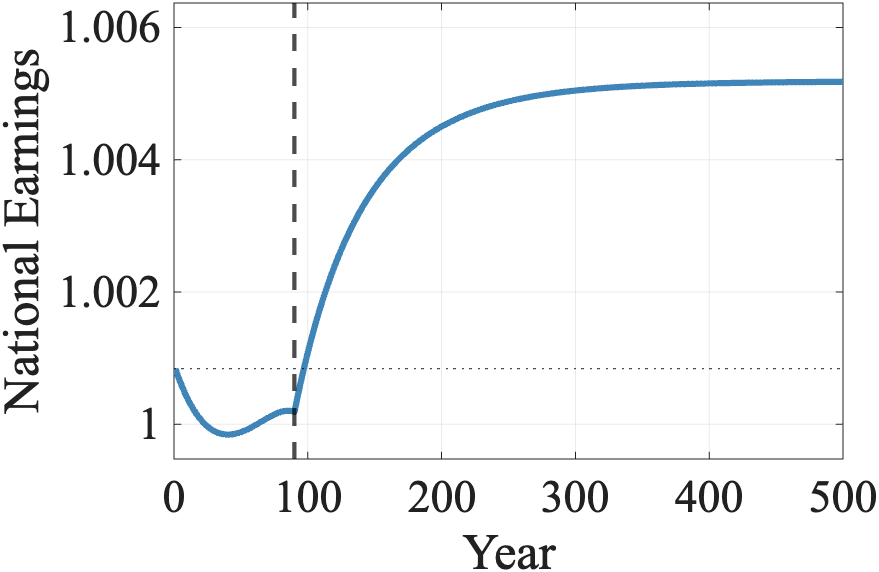
\includegraphics[width=\textwidth]{../Output/big_nu/graph_perfect_foresight/dynamic_moments/dynamic_moments_national_earnings.png}
  \end{minipage}\hfill
  \begin{minipage}[t]{0.24\textwidth}
    \centering
    \small{(b) Mobility}
    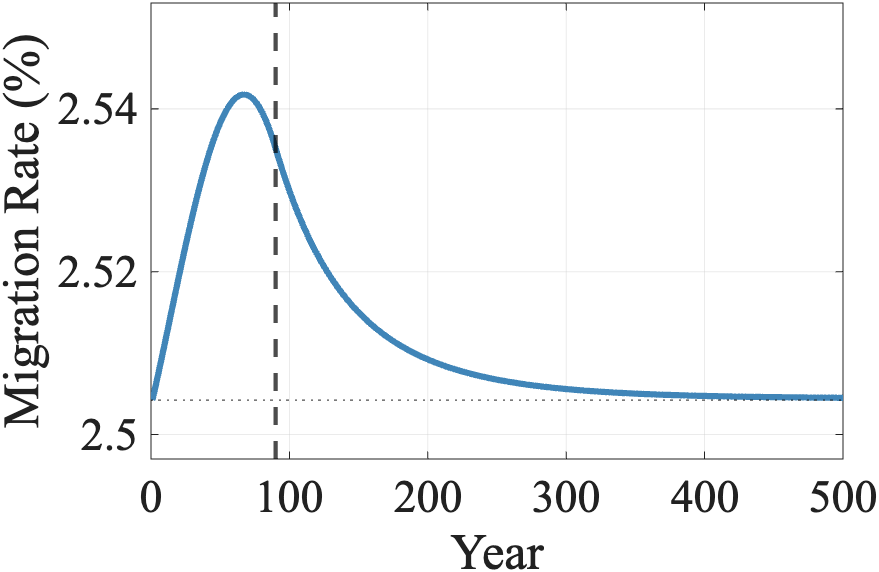
\includegraphics[width=\textwidth]{../Output/big_nu/graph_perfect_foresight/dynamic_moments/dynamic_moments_national_mobility.png}
  \end{minipage}\hfill
  \begin{minipage}[t]{0.24\textwidth}
    \centering
    \small{(c) Wealth}
    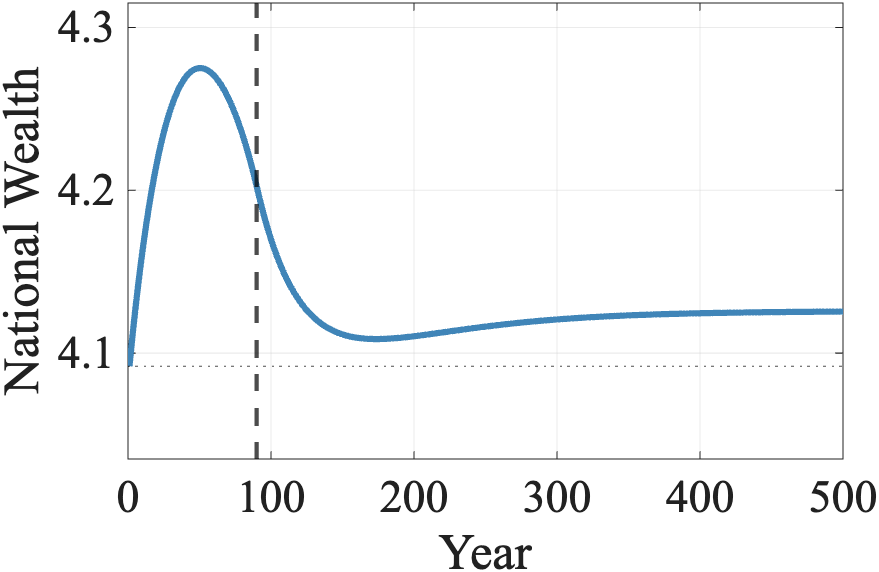
\includegraphics[width=\textwidth]{../Output/big_nu/graph_perfect_foresight/dynamic_moments/dynamic_moments_national_wealth.png}
  \end{minipage}\hfill
  \begin{minipage}[t]{0.24\textwidth}
    \centering
    \small{(d) W/Y Ratio}
    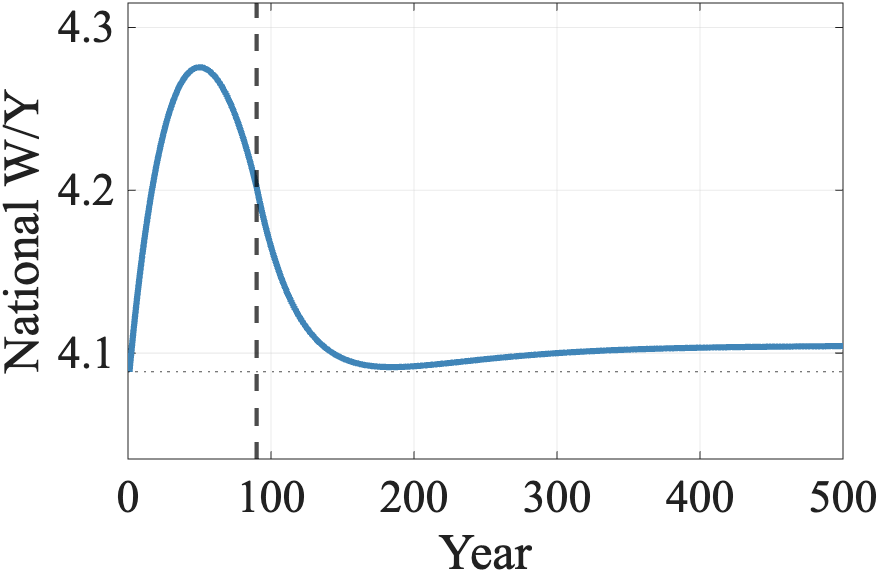
\includegraphics[width=\textwidth]{../Output/big_nu/graph_perfect_foresight/dynamic_moments/dynamic_moments_national_wy.png}
  \end{minipage}
  \begin{minipage}{\textwidth}
  \vspace{0.4em}
  \footnotesize{\textbf{Note:} Aggregate macroeconomic time series under Perfect Foresight, 2010--2500+. Panel (a): national total disposable labour earnings $Y_t = \sum_{\ell=1}^J \tilde{w}_{\ell,t} (L_{\ell,t} + \int z \Lambda_t(\ell,z)\,\mathrm{d}z)$. Panel (b): national gross annual inter-state migration rate $m_t = \sum_{\ell=1}^J \int \Lambda_t(\ell,z) [1 - \mu_{\ell \ell,t}(z)]\,\mathrm{d}z / \sum_\ell L_{\ell,t}$. Panel (c): total national wealth holdings $W_t = \sum_{\ell=1}^J \int \bar{a}_t(\ell,z) \Lambda_t(\ell,z)\,\mathrm{d}z$. Panel (d): aggregate wealth-to-earnings ratio $(W/Y)_t = W_t / Y_t$, capturing precautionary asset accumulation ahead of climate shocks and subsequent decumulation.}
  \end{minipage}
\end{figure}

\subsection{Spatial Differences Across the Two Steady States}
Comparing the initial and final steady states reveals the spatial heterogeneity that is hidden by national aggregates. The model predicts a strong North-South gradient in population reallocation: the South-East experiences an important drop in population, most notably a local population decline of 80\% in Florida and 20 to 30\% across the broader region, while the North-East and specific northern states like Alaska see local population go up by 20 to 30\% and up to 60 percent, respectively. 
This spatial gradient is similar when looking at the wealth accumulation and the wealth-to-income ratio. States such as Florida and Louisiana experience a drop in mean wealth of approximately 25 percent, contrasted with increases of over 10\% in states like Montana and Oregon. The spatial distribution of these effects is not symmetric: the magnitude of local economic drop in the more affected regions is larger than the expansions in the other states. National aggregates fail to capture this asymmetry due to the weighting effect: heavily damaged states like Florida lose over 70\% of their population so their contribution to the national aggregate wealth shrinks, masking the severity of wealth destruction. Furthermore, while the decline in local wages correlates with a decline in wealth, the proportional drop in wealth systematically exceeds the drop in wages, driving the wealth-to-income ratio down in tandem with per-state mean wealth. 

\begin{figure}[!htb]
  \centering
  \caption{Transition Maps (Perfect Foresight)}
  \label{fig:trans_map_pf}
  \begin{minipage}[t]{0.32\textwidth}
    \centering
    \small{(a) $\Delta$ W/Y Ratio in level}
    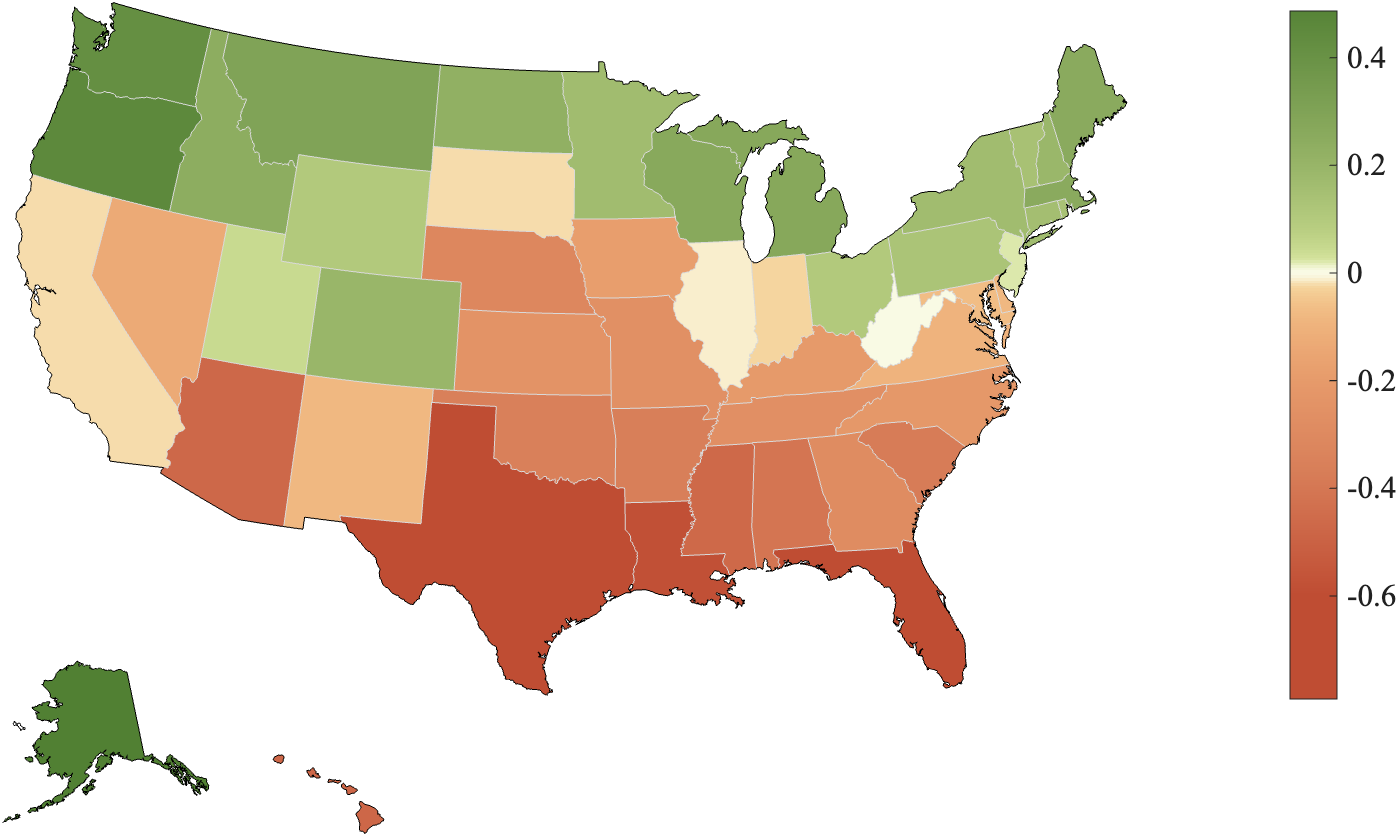
\includegraphics[width=\textwidth]{../Output/big_nu/graph_perfect_foresight/transition_maps/transition_maps_wealth_income_ratio_changes.png}
  \end{minipage}\hfill
  \begin{minipage}[t]{0.32\textwidth}
    \centering
    \small{(b) $\Delta$ Local Population (\%)}
    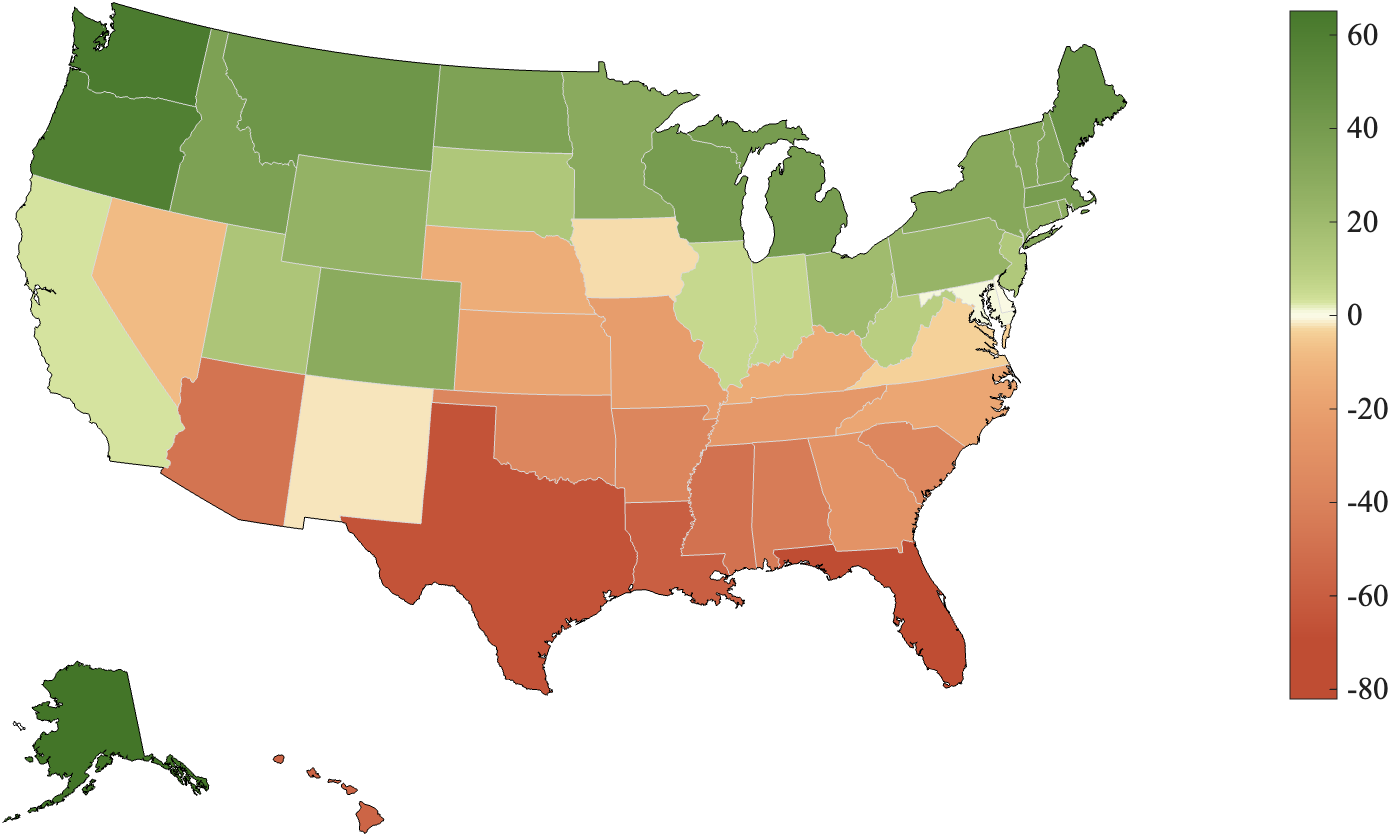
\includegraphics[width=\textwidth]{../Output/big_nu/graph_perfect_foresight/transition_maps/transition_maps_local_pop_changes_pct.png}
  \end{minipage}\hfill
  \begin{minipage}[t]{0.32\textwidth}
    \centering
    \small{(c) $\Delta$ Mean Wealth (\%)}
    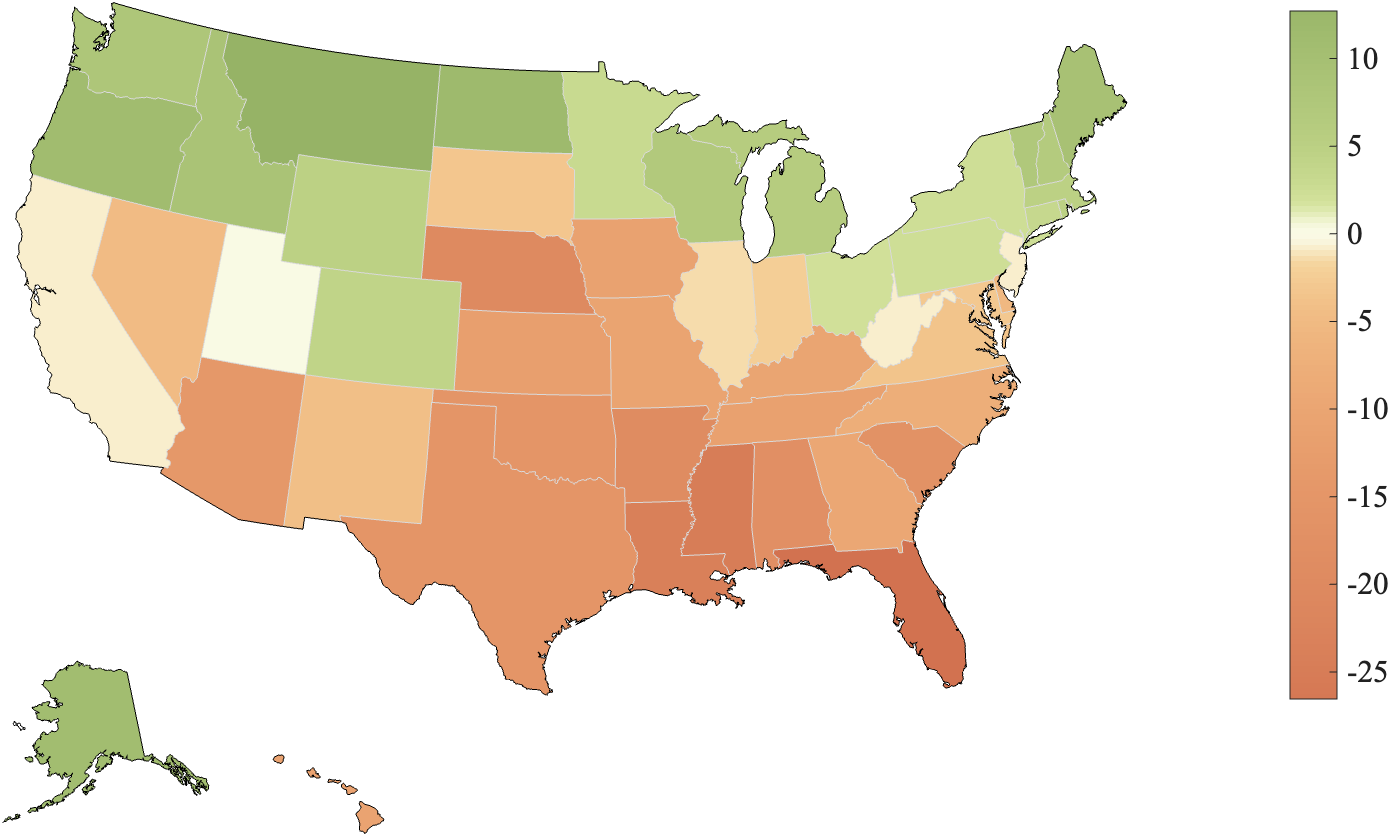
\includegraphics[width=\textwidth]{../Output/big_nu/graph_perfect_foresight/transition_maps/transition_maps_pop_changes_pp.png}
  \end{minipage}
  \begin{minipage}{\textwidth}
  \vspace{0.5em}
  \footnotesize{\textbf{Note:} Spatial maps comparing the terminal steady state under 2100 climate parameters ($SS_\text{term}$) to the initial 2010 baseline steady state ($SS_\text{init}$) under Perfect Foresight. Panel (a): change in state wealth-to-earnings ratio $\Delta (W/Y)_\ell = (W/Y)_{\ell, \text{term}} - (W/Y)_{\ell, \text{init}}$. Panel (b): relative population percentage change $\Delta L_\ell\% = 100 \times (L_{\ell, \text{term}} - L_{\ell, \text{init}})/L_{\ell, \text{init}}$. Panel (c): percentage change in state mean per-capita wealth $\Delta \bar{a}_\ell\%$.}
  \end{minipage}
\end{figure}

Why do mean wealth and the wealth-to-income ratio drop so sharply in damaged Southern states while rising in Northern havens? The next section derives the analytical saving motives and decomposes these regional shifts.

\FloatBarrier
\section{Unpacking Wealth Dynamics}
\label{sec:mechanisms}
\subsection{Analytical Saving Motives}
\label{sec:saving_motives}
I decompose the saving rule $\Delta a_{t+1} = a_{t+1} - a_t$ by sequentially introducing the model's mechanisms.
\subsubsection*{Deterministic Fundamentals: Permanent Income and Amenity Smoothing}
In a scenario where spatial mobility is shut down ($J=1$) and the idiosyncratic income process is turned off, accumulation is driven by the anticipation of future changes in local fundamentals.  

Let us define the Permanent Income $y_t^P$ and the Permanent Amenity $A_t^P$ as the annuity values of their respective future streams:
\begin{align}
    y_t^P &= \frac{r}{1+r} \sum_{s=0}^{\infty} \frac{\tilde{y}_{t+s}}{(1+r)^s}, &
    A_t^P &= \frac{r}{1+r} \sum_{s=0}^{\infty} \frac{\tilde{A}_{t+s}}{(1+r)^s}. \label{eq:perm_income}
\end{align}
The individual saving rule can be then written as:\footnote{For clarity the impatience related term $\log(\beta(1+r))$ is omitted. It is also motivated by the calibration of the model where $\beta = 1/(1+r)$, making the impatience term equal to zero.}
\begin{equation}
    \Delta a_{t+1} = (1+r) \left( \tilde{y}_t - y_t^P \right) + \frac{1+r}{\gamma} \left( \tilde{A}_t - A_t^P \right)
    \label{eq:saving_permanent}
\end{equation}
Equation (\ref{eq:saving_permanent}) illustrates two distinct precautionary motives. The first term represents the standard Permanent Income Hypothesis (PIH): workers save if their current disposable income exceeds their permanent income. The second term introduces an amenity smoothing mechanism: if current amenities are superior to the permanent amenity level, workers accumulate additional savings today to finance higher future consumption, compensating for the anticipated loss in local quality of life. 

Let the baseline pre-shock fundamentals $w, q,$ and $A$ be constant, and define the incremental climate damage occurring between period $t$ and $t+1$ as $\Delta D_{t+1} = D_{t+1} - D_t$. Equation (\ref{eq:saving_permanent}) yields the present discounted value of all future fundamental degradations:
\begin{equation}
    \Delta a_{t+1} = \sum_{s=0}^{\infty} \frac{1}{(1+r)^s} \left[ \underbrace{w \Delta D^w_{t+s+1}}_{\text{Wage loss}} + \underbrace{q \Delta D^q_{t+s+1}}_{\text{Housing cost rise}} + \underbrace{\frac{1}{\gamma} \Delta D^A_{t+s+1}}_{\text{Monetised amenity loss}} \right]
    \label{eq:saving_climate}
\end{equation}
In Equation~(\ref{eq:saving_climate}), should the climate stabilise and damages reach a permanent plateau ($\Delta D = 0$), precautionary accumulation ceases ($\Delta a_{t+1} = 0$). This damage-ramp smoothing ($\Delta D > 0$ over 2010--2100, $\Delta D = 0$ thereafter) generates the $+4.5$\% transitional surge in national wealth observed in Figure~\ref{fig:trans_dyn_pf}.
\subsubsection*{Idiosyncratic Income Risk: Precautionary Savings}
When I reintroduce the uninsurable idiosyncratic income process (composed of a persistent AR(1) component $z$ and a transitory component $\eta$) the deterministic framework extends to a stochastic one. Let $\tilde{Y}_{t+s} = \tilde{y}_{t+s} + \tilde{w}_{t+s} z_{t+s} + \tilde{w}_{t+s} \eta_{t+s}$ denote the total disposable income. The PIH term is now evaluated using the conditional expectation $\mathbb{E}_t[\tilde{Y}_{t+s}]$. Furthermore, the uninsurable risk generates a positive precautionary saving motive. Let $\sigma_{C, t+s}^2$ denote the variance of the innovation to permanent income occurring at period $t+s$, which aggregates both the transitory shock $\eta$ and the persistent shock $\epsilon$:
\begin{equation}
    \sigma_{C, t+s}^2 = \left( \frac{r}{1+r} \tilde{w}_{t+s} \right)^2 \sigma_{\eta, t+s}^2 + \Omega_{t+s}^2 \sigma_{\epsilon, t+s}^2
    \label{eq:var_innovation}
\end{equation}
where $\Omega_{t+s} = \frac{r}{1+r} \sum_{k=0}^{\infty} \frac{\rho^k \tilde{w}_{t+s+k}}{(1+r)^k}$ translates a unit persistent shock $\epsilon_{t+s}$ into a permanent flow.
Using a summation by parts on the conditional expectations, the saving equation generalises to include risk:
\begin{equation}
    \Delta a_{t+1}(z) = \sum_{s=0}^{\infty} \frac{1}{(1+r)^s} \left[ \underbrace{\left(\mathbb{E}_t[\tilde{Y}_{t+s}] - \mathbb{E}_t[\tilde{Y}_{t+s+1}]\right)}_{\text{Expected Income Drop}} + \underbrace{\frac{1}{\gamma} (\tilde{A}_{t+s} - \tilde{A}_{t+s+1})}_{\text{Amenity Drop}} + \underbrace{\textcolor{mutedgold}{\frac{\gamma}{2} \sigma_{C, t+s+1}^2}}_{\textcolor{mutedgold}{\text{Precautionary Risk}}} \right]
    \label{eq:saving_stochastic}
\end{equation}

I can decompose the expected income drop to separate the climate damages from the idiosyncratic mean-reversion. Knowing that $\mathbb{E}_t[z_{t+s}] = \rho^s z_t$ and that effective wages evolve as $\tilde{w}_{t+s+1} = \tilde{w}_{t+s} - w \Delta D^w_{t+s+1}$, I can expand the income drop into three distinct economic forces:
\begin{equation}
    \mathbb{E}_t[\tilde{Y}_{t+s}] - \mathbb{E}_t[\tilde{Y}_{t+s+1}] = \underbrace{w \Delta D^w_{t+s+1} (1 + z_t \rho^{s+1}) + q \Delta D^q_{t+s+1}}_{\text{Net Climate Damage Drop}} + \underbrace{z_t \rho^s (1 - \rho) w}_{\text{ Mean-Reversion}} - \underbrace{\textcolor{terracotta}{z_t \rho^s (1 - \rho) w D^w_{t+s}}}_{\textcolor{terracotta}{\text{Damage-Level Dampening}}}
    \label{eq:income_drop_decomp}
\end{equation}
It shows how climate change alters income expectations on two distinct margins: the growth of damages ($\Delta D$) increases the expected income drop, while the level of accumulated damages ($D$) dampens the absolute monetary value of standard idiosyncratic mean-reversion. Because the base wage drops, the absolute dollar value of any given percentage income shock decreases, dampening both the expected mean-reversion and the absolute monetary risk $\sigma_C^2$ (reducing $\Omega$). If climate change increases the variance of future transitory shocks, the augmentation in $\sigma_{\eta, t+s}^2$ increases $\sigma_C^2$, accelerating precautionary wealth accumulation.
\subsubsection*{Spatial Mobility: Substitutability and Complementarity}
In the environment with migration ($J > 1$) but without idiosyncratic income risk, a $\log$ transformation of Equation~\ref{eq:mu} expresses the inclusive value through the probability of staying in the origin location, $\mu_{\ell \ell, t}$. Since $\psi_{\ell\ell} = 0$, solving recursively for the saving policy rule along the path where the agent stays in location $\ell$ yields:\footnote{The constant shift $\ln\bar{\lambda}/\gamma$ induced by the Weibull mean is omitted for clarity.}
\begin{equation}
    \Delta a_{\ell, t+1} = \sum_{s=0}^{\infty} \frac{1}{(1+r)^s} \left[ \underbrace{(\tilde{y}_{\ell, t+s} - \tilde{y}_{\ell, t+s+1}) + \frac{1}{\gamma} (\tilde{A}_{\ell, t+s} - \tilde{A}_{\ell, t+s+1})}_{\text{Local Climate Damage Smoothing}} + \underbrace{\textcolor{emerald}{\frac{1}{\gamma \nu} \ln \mu_{\ell  \ell, t+s}}}_{\textcolor{emerald}{\text{Option Value of Spatial Insurance}}} \right]
    \label{eq:saving_spatial}
\end{equation}
Because $\mu_{\ell \ell, t+s}$ is a probability ($\mu \le 1$), its logarithm is non-positive ($\ln \mu \le 0$). The ability to spatially reallocate acts as an insurance mechanism, substituting for the accumulation of financial wealth and reducing the need to save compared to autarky.

Equation (\ref{eq:saving_spatial}) reveals a relationship of both substitutability and complementarity between spatial mobility and saving. First, spatial mobility acts as a substitute for savings, but its effect is asymmetric across locations. In damaged states, local economic fundamentals drop, causing the option value of leaving to go up: workers rely more on the migration network to escape. For states that are relatively untouched by damages, local fundamentals remain strong, but the global degradation of outside options puts the spatial option value ($\mu_{\ell \ell}$) closer to 1, diminishing the option value term to $\ln \mu_{\ell \ell} \to 0$. Without this spatial insurance, workers are forced to substitute towards saving. Second, idiosyncratic preference shocks ($\varepsilon$) generate a complementary demand for wealth. In a post-shock equilibrium, drawing a strong spatial preference often requires migrating to a destination with degraded economic fundamentals. To absorb this drop in income without enduring a drop in consumption, workers require accumulated wealth. In this sense, savings act as a complement to spatial mobility, financing the realisation of location preferences in a climate-damaged world.

\subsection{Steady-State Wealth Decomposition}
\label{sec:wealth_decomp}
Because climate fundamentals are constant within any steady state ($\Delta D = 0$), the transitional permanent income smoothing motive vanishes when comparing different steady states. The change in average local wealth is then governed by three distinct margins: a behavioural adjustment, the spatial change of historical wealth, and a compositional sorting.
\paragraph{Saving Rule.} With the Blanchard-Yaari demographic structure, the steady-state target wealth for a worker of productivity $z$ who remains in location $\ell$ is an equilibrium stock proportional to the flow of the remaining stationary saving motives, scaled by the demographic survival multiplier. The intensive shift in this behavioural savings policy, denoted $\Delta a_\ell^{\text{Saving Rule}}(z)$, is driven by the cross-steady-state shift in these motives:
\begin{equation}
    \Delta a_\ell^{\text{Saving Rule}}(z) \propto \sum_{s=0}^{\infty} \frac{1}{(1+r)^s} \left[ \underbrace{\textcolor{terracotta}{- z \rho^s (1-\rho) w \Delta^{SS} D^w_\ell}}_{\textcolor{terracotta}{\text{Damage-Level Dampening}}} + \underbrace{\textcolor{mutedgold}{\frac{\gamma}{2} \Delta^{SS} \sigma_{C, \ell}^2}}_{\textcolor{mutedgold}{\Delta \text{Precautionary Risk}}} + \underbrace{\textcolor{emerald}{\frac{1}{\gamma \nu} \Delta^{SS} \ln \mu_{\ell \ell}(z)}}_{\textcolor{emerald}{\Delta \text{Spatial Option Value}}} \right]
    \label{eq:intensive_margin_decomposition}
\end{equation}
\paragraph{Spatial Transition (Historical Origin).}
Even if the local saving policy (Equation~\ref{eq:intensive_margin_decomposition}) remained constant, average wealth would shift due to a spatial transition margin, denoted $\Delta a_\ell^{\text{Transition}}(z)$. This margin captures the change in the historical origins of the population: as climate change alters the migration network, the workers arriving in $\ell$ today come from different locations, bringing different levels of past wealth and saving rules.
\paragraph{Compositional Sorting.}
The average per-capita wealth in location $\ell$ is the expectation over the productivity distribution: $\bar{a}_\ell = \int \pi_\ell(z) a_\ell(z)\,\mathrm{d}z$, where $\pi_\ell(z)$ is the stationary density of workers of type $z$ residing in $\ell$. To separate these wealth changes from demographic reallocations, the total state-level wealth variation is decomposed as:
\begin{equation}
    \Delta^{SS} \bar{a}_\ell = \int \pi_\ell^{\text{init}}(z) \Big[\Delta a_\ell^{\text{Saving Rule}}(z) + \underbrace{\textcolor{lightemerald}{\Delta a_\ell^{\text{Transition}}(z)}}_{\textcolor{lightemerald}{\text{Spatial Transition}}} \Big]\,\mathrm{d}z + \underbrace{\textcolor{cobaltblue}{\int \big[\pi_\ell^{\text{term}}(z) - \pi_\ell^{\text{init}}(z) \big] a_\ell^{\text{term}}(z)\,\mathrm{d}z}}_{\textcolor{cobaltblue}{\text{Compositional Sorting}}}
    \label{eq:wealth_decomposition}
\end{equation}

\paragraph{Empirical Decomposition.} To disentangle these five mechanisms empirically (damage-dampening, precautionary risk, spatial option value, spatial transition, and compositional sorting) Figure~\ref{fig:trans_wy_pf} applies this decomposition across states.\footnote{More details for the computation of the decomposition are given in Appendix~\ref{app:algorithms}.} The decomposition yields several insights. First, the risk effect is quantitatively negligible. The vast majority of the heterogeneity in wealth dynamics is driven by the three spatial components. In particular, the spatial option effect, which captures shifts in migration probabilities and implicit changes in non-market amenities, is the primary driver of changes in wealth across steady states. As theorised in Subsection~\ref{sec:saving_motives}, workers in states like Alaska or Oregon accumulate additional precautionary wealth to insure against the risk of drawing an idiosyncratic shock that would make them migrate to a climate-damaged state. On the other side of the table, in severely impacted states like Florida or Louisiana, the spatial option effect suppresses wealth accumulation. Workers in these regions anticipate that conditional on drawing a sufficiently large preference shock to migrate, they will likely relocate to a state with superior wages or amenities, thus reducing their current precautionary savings motive.

Then, the spatial transition effect accounts for changes in wealth driven by shifts in the historical origins of a state's population that is governed by the interaction between moving cost and the geographic distribution of climate damages. The average wealth in adjacent states (that are for the most part also hit by climate change) is dragged down, as their incoming migration comes more often from damaged neighbouring states. For relatively undamaged states, the spatial transition effect is often positive. Because their fundamental value rises relative to the rest of the country $\mu_{jj}$ increases for those states. By having a larger share of their  residents and proportionally fewer immigrants, the historical origin of these safe states shifts towards higher average wealth. For instance, severely damaged states with historically low baseline wealth (such as Louisiana) can exhibit a positive spatial transition effect: their population flees and the remaining population comes from states that are historically wealthier. The attractive states that are relatively close to the damaged states (such as Montana) can exhibit a negative transition effect if they experience an influx of immigrants whose origin-state wealth is lower than the haven's baseline.

Finally, the compositional sorting effect isolates the change in wealth attributable to the endogenous spatial sorting of productivity types. Severely impacted states like Florida and Louisiana lose high-productivity workers who save more than the other workers (mainly because they are more prone to mean-reverting saving), which reduces the mean productivity and mean wealth in those states. States like Alaska and Oregon experience the reverse, absorbing high-productivity workers and thereby increasing their mean wealth.
\input{figures/trans_wy_pf.tex}

\FloatBarrier
\section{Counterfactuals and Welfare Analysis}
\label{sec:counterfactuals}
Having examined the baseline transition and the channels driving regional wealth divergence, I turn to counterfactual scenarios that vary expectations or shut down each adaptation margin. In the Myopia scenario, agents are unaware of future trajectories and base their decisions on current conditions. In the No Migration scenario, migration costs are set to $\psi_{j\ell} = 10^8$ for $j \neq \ell$, shutting down interstate mobility; in the No Saving scenario, agents are not allowed to save.

\subsection{Counterfactual 1: Forward-Looking Anticipation (Myopia)}
\label{sec:myopia}
\paragraph{Shutting Down Anticipation.} In the Myopia scenario, agents base decisions on current conditions, ignoring the expected trajectory of wages and amenities.\footnote{The algorithm therefore solves the fixed point of Equation~\ref{eq:Xi} at each period independently; see Appendix~\ref{app:algorithms}.} Note that without perfect foresight, the economy still reaches the same terminal steady state, but via a different transition path. Figure~\ref{fig:welfare_comp_pc}(a) displays the wealth-to-income trajectory for the Myopia scenario.

Aggregate earnings and the inter-state migration rate follow roughly the same trajectory as in the baseline scenario, only with a slight delay (the migration rate peaks in 2100 in the Myopia scenario, compared to 2090 in the baseline). More importantly, because there is no anticipation of future damages, agents do not engage in precautionary saving to smooth the expected gradual drop in wages and amenities. As agents are hit by progressive climate damages that they fail to anticipate, they treat each successive deterioration as an unexpected, permanent shock, forcing them to consume out of their wealth rather than accumulate savings in anticipation. After 2100, once climate fundamentals stabilise, workers find their asset holdings are below the new steady-state target. They must gradually increase their saving rate to rebuild their precautionary saving, causing aggregate wealth and the wealth-to-income ratio to slowly recover towards the new steady state. 

Finally, the speed of convergence to the new steady state is significantly slower under myopia. The transition takes approximately 400 periods (years), compared to 300 periods in the baseline scenario.

\subsection{Counterfactual 2: Suppressing Spatial Mobility (Autarky)}
\label{sec:margins}

\paragraph{Shutting Down Migration.} In the No Migration scenario, I set the bilateral migration costs to be prohibitively high ($\psi_{j\ell} = 10^8$ for $j \neq \ell$), effectively preventing any interstate migration. Methodologically, I maintain the same initial steady state with active migration as the baseline. The economy then transitions along two distinct paths: a control path with no migration and no climate change, and a treatment path with no migration but incorporating climate change. This Difference-in-Differences (DiD) approach isolates the effect of climate change under autarky and ensures that all counterfactual outcomes are evaluated against a consistent initial benchmark. As explained in Section~\ref{sec:mechanisms}, in the no-climate control path shutting down spatial insurance causes the aggregate wealth-to-income ratio to surge from 4.1 to 7.3.


\paragraph{National aggregates.} Wealth-to-income dynamics are shown in Figure~\ref{fig:welfare_comp_pc}(a). The migration rate is zero by construction, and aggregate earnings drop by 1.1 percent, reflecting the population-weighted average of the wage shock across states. Because agents cannot rely on relocating to less affected states, they accumulate more wealth to self-insure against the anticipated decline in wages and amenities: the wealth-to-income ratio peaks at $+6\%$ above the no-climate control path before 2100, compared to $+4.5\%$ in the baseline (Figure~\ref{fig:welfare_comp_pc}(a)). Because there is no reallocation of population towards more productive states in the terminal steady state, the wealth-to-income ratio declines in the long run.

\begin{figure}[htb]
  \centering
  \caption{Transition Map (No Migration): $\Delta$ Mean Wealth (\%)}
  \label{fig:spatial_hetero_no_migration}
  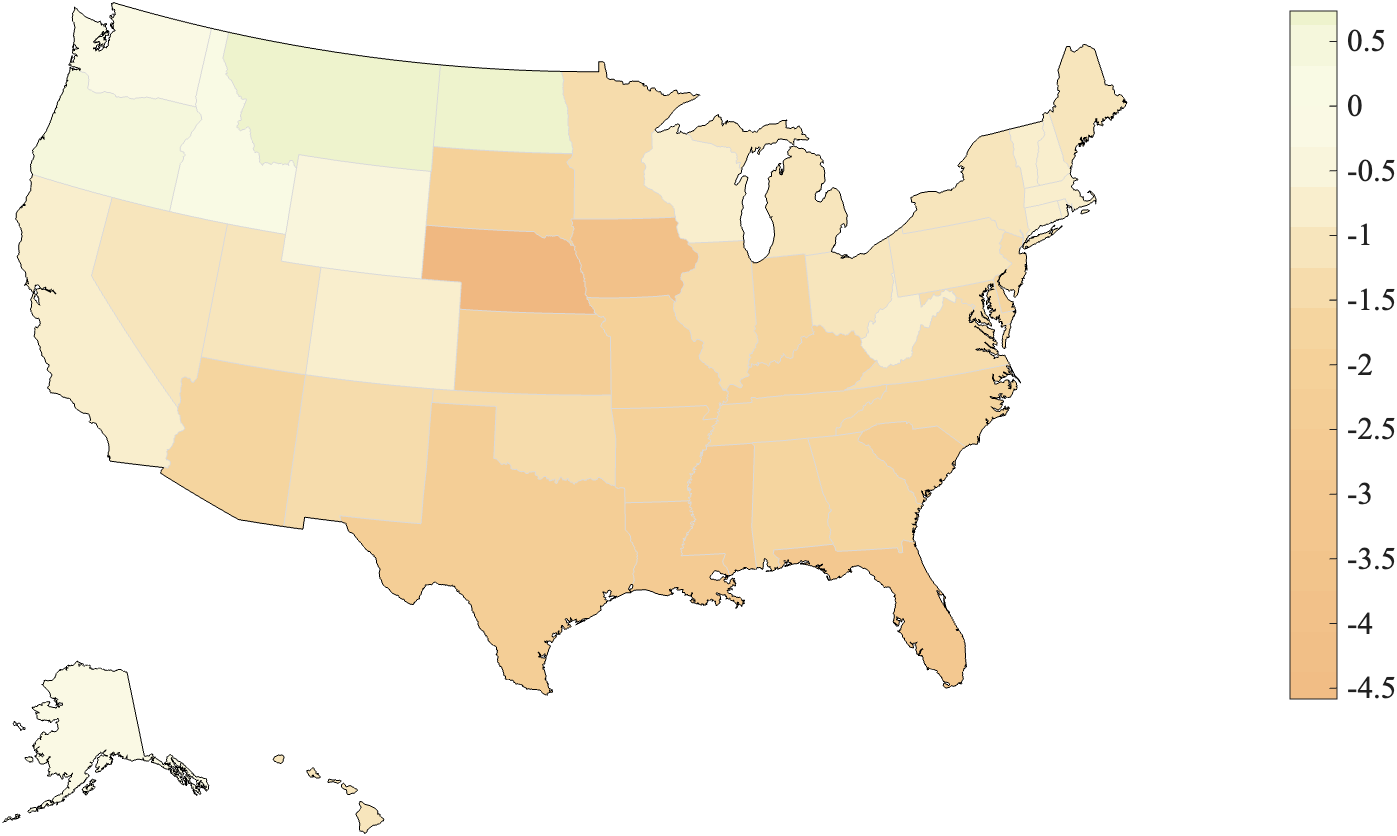
\includegraphics[width=0.55\textwidth]{../Output/big_nu/graph_no_migration_did/transition_maps/transition_maps_pop_changes_pp.png}
  \begin{minipage}{\textwidth}
  \vspace{0.5em}
  \footnotesize{\textbf{Note:} Spatial map comparing the terminal steady state under 2100 climate parameters ($SS_\text{term}$) to the initial 2010 baseline steady state ($SS_\text{init}$) under No Migration autarky ($\Delta L_\ell\% \equiv 0$): percentage change in state mean per-capita wealth $\Delta \bar{a}_\ell\%$.}
  \end{minipage}
\end{figure}

\paragraph{Spatial heterogeneity.} Results are presented in Figure~\ref{fig:spatial_hetero_no_migration}. The absence of migration prevents the spatial sorting of workers based on productivity and amenities, and eliminates the influence of idiosyncratic preference shocks on spatial reallocation. The spatial option value, transition, and composition margins are entirely absent. Changes in wealth are driven uniquely by the damage-dampening and risk margins, which affect states more uniformly.


\FloatBarrier
\subsection{Counterfactual 3: Suppressing Wealth Accumulation (Hand-to-Mouth)}
\paragraph{Shutting Down Saving} To evaluate the counterfactual scenario in which the saving mechanism is suppressed, I construct a variant of the model where agents operate as hand-to-mouth consumers. This modification is necessary because the closed-form resolution of the baseline model relies on the Euler equation that governs the optimal consumption-saving path. The unique change lies in the derivation of the continuation value, $\Xi_{\ell,t}(z^\prime)$, which is reconstructed to evaluate lifetime expected utility under the binding constraint that current income must be allocated to today's consumption. In this scenario, worker asset holdings $a$ are zero, and the Certainty Equivalent adjustment drops the wealth term.

In this hand-to-mouth specification, workers consume their full disposable income each period: $c_{\ell,t} = \tilde{y}_{\ell,t} + \tilde{w}_{\ell,t}z^\prime + \tilde{w}_{\ell,t}\eta^\prime$. Substituting this into the intra-period utility and applying the expectation operator over the transitory shock $\eta^\prime$, the new recursive continuation value is:
\begin{equation}
\Xi_{\ell,t}(z^\prime) = -\frac{1}{\gamma} \ln \left( \exp\left(F_{\ell,t}(z^\prime)\right) + \beta \Omega_{\ell,t}(z^\prime) \right)
\label{eq:Xi_nosaving}
\end{equation}
where $F_{\ell,t}(z^\prime) = -\gamma \tilde{y}_{\ell,t} - \gamma \tilde{w}_{\ell,t} z^\prime - \tilde{A}_{\ell,t} + \frac{1}{2}(\gamma \tilde{w}_{\ell,t})^2 \sigma_{\eta,\ell}^2$ is the flow utility from consuming today's income, and $\Omega_{\ell,t}(z^\prime) = \bar{\lambda} \left[ \frac{1}{J} \sum_{m=1}^J e^{-\nu \psi_{\ell m}} \left( \mathbb{E}_{z^{\prime\prime}|z^\prime, m} \left[ e^{-\gamma \Xi_{m,t+1}(z^{\prime\prime})} \right] \right)^{-\nu} \right]^{-1/\nu}$ is the spatial value capturing the option to migrate in the subsequent period, incorporating the extreme value preference shocks. Although individual migration probabilities $\mu_{j\ell,t}(z)$ are independent of current asset holdings $a$ in the baseline consumer problem, suppressing saving alters migration behaviour through an indirect channel: without intertemporal consumption smoothing, uninsurable local income risk enters the continuation value $\Xi_{\ell,t}(z^\prime)$ unbuffered, reshaping destination values and equilibrium mobility flows. The full derivation of Equation~\eqref{eq:Xi_nosaving} is provided in Appendix~\ref{app:proofs}.

\paragraph{National Aggregate.} In the initial steady state, with no saving both the population distribution and the interstate migration rate change: earnings are on average lower, meaning that more people live in poorer states, which happen to be Southern States. The aggregate migration rate stands at 2.7\%, higher than the baseline. This reflects substitutability between saving and migration. Without the ability to save and thereby smooth consumption variance from idiosyncratic income shocks, workers are forced to rely on spatial mobility to smooth shocks, increasing the inter-state mobility rate. The inter-state mobility rate peaks in 2090 at roughly 2.75\% before settling at a higher terminal value. This permanent increase is driven by a compositional shift in the population. In the No Saving economy, high-wage Northern states impose a higher uninsurable variance penalty ($\frac{1}{2}(\gamma \tilde{w}_{\ell,t})^2 \sigma_{\eta,\ell}^2$) than the baseline, making them high-turnover regions. As climate damages force population out of the Southern states and into higher-variance Northern and middle states, the national aggregate migration rate rises because a larger share of the population lives in high-turnover environments.

\paragraph{Spatial Heterogeneity.} The heterogeneity in population change is shown in Figure~\ref{fig:spatial_hetero_no_saving}. The magnitude of population reallocation is visually less pronounced in the No Saving scenario (e.g., Florida loses approximately 60\% of its population, compared to 80\% in the baseline, while Northern states see less influx). The smaller percentage drop in the South is the result of the initial population distribution: the No Saving scenario begins with a higher Southern population base, meaning an identical absolute migratory outflow yields a smaller relative percentage decline. Second, the missing population influx to the North is driven by the uninsurable variance penalty. In a hand-to-mouth environment, agents must consume their entire income, forcing them to bear the full income variance: $\frac{1}{2}(\gamma \tilde{w}_{\ell,t})^2 \sigma_{\eta,\ell}^2$. Because this uninsurable risk premium scales with the square of the local wage, more productive Northern states become less attractive. When climate refugees flee the South, this variance penalty acts as a barrier to entry for high-wage havens, forcing migrants to disperse across sub-optimal, lower-variance states and dampening the aggregate directional reallocation.

\begin{figure}[!htb]
  \centering
  \caption{Transition Map (No Saving): $\Delta$ Local Population (\%)}
  \label{fig:spatial_hetero_no_saving}
  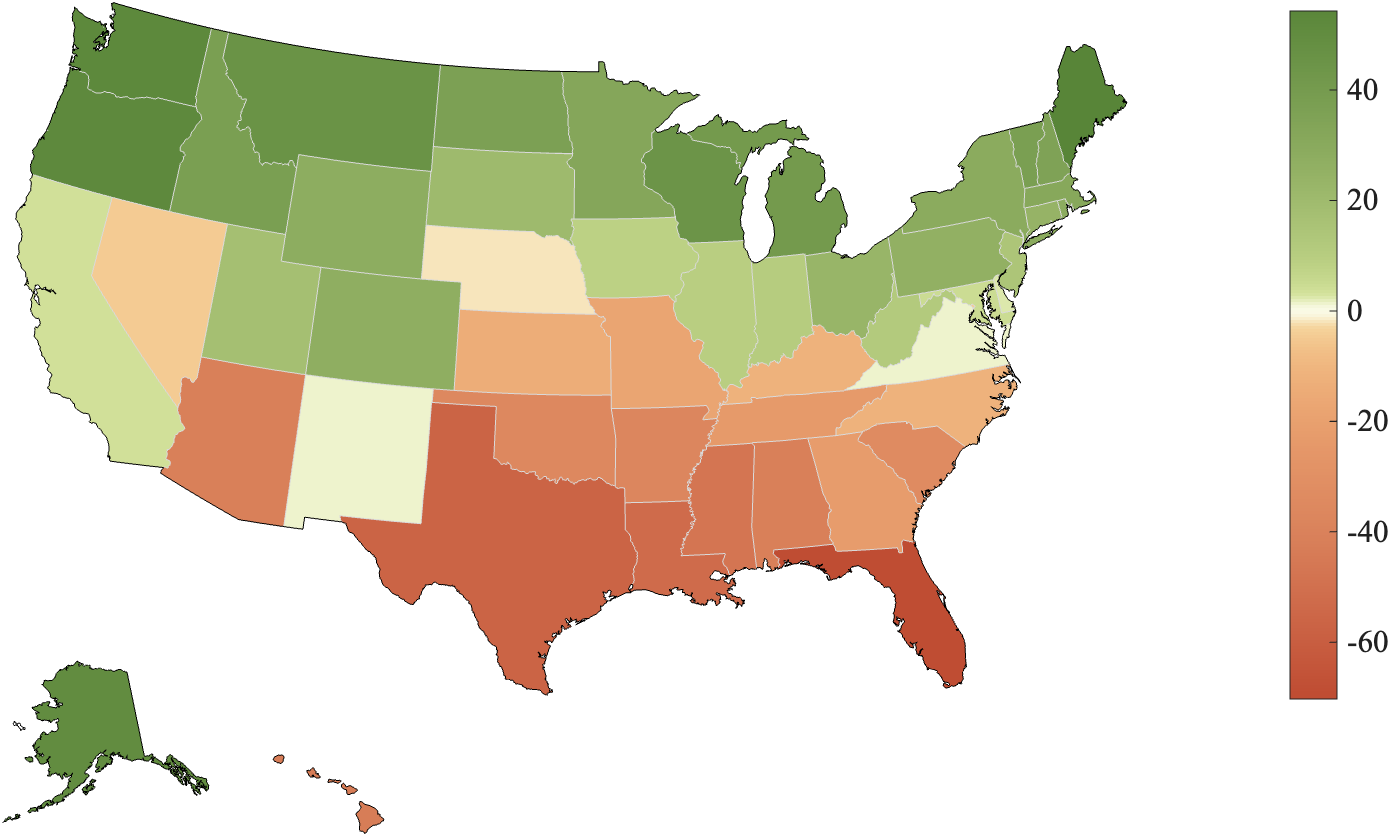
\includegraphics[width=0.52\textwidth]{../Output/big_nu/graph_no_saving_struct/transition_maps/transition_maps_local_pop_changes_pct.png}
  \begin{minipage}{\textwidth}
  \vspace{0.5em}
  \footnotesize{\textbf{Note:} Spatial map comparing the terminal steady state under 2100 climate parameters ($SS_\text{term}$) to the initial 2010 baseline steady state ($SS_\text{init}$) under Hand-to-Mouth workers: relative population percentage change $\Delta L_\ell\% = 100 \times (L_{\ell, \text{term}} - L_{\ell, \text{init}})/L_{\ell, \text{init}}$.}
  \end{minipage}
\end{figure}

\FloatBarrier
\subsection{Welfare Evaluation and Cross-Scenario Analysis}
\label{sec:audit}
\paragraph{Welfare metric.} The Certainty Equivalent of a worker in location~$\ell$ with persistent productivity state $z$ and assets $a$ is defined in consumption units as:
\begin{equation}
    CE_t(\ell, z, a) \;=\; \frac{1}{1+r}\, a \;+\; \Xi_{\ell,t}(z).
\end{equation}
Defining initial steady-state material flow consumption in state $\ell$ as $c^{\text{init}}_{\ell} \equiv \tilde{y}^{\text{init}}_\ell + \frac{r}{1+r}\,\bar{a}^{\text{init}}(\ell)$, the national Consumption Equivalent Variation is:
\begin{equation}\label{eq:lambda_nat}
    \frac{\displaystyle\sum_{\ell=1}^{J} \bigl(\overline{CE}_t(\ell) - \overline{CE}^{\,\text{init}}(\ell)\bigr)\, L_{\ell,t}}{\displaystyle\sum_{\ell=1}^{J}\, c^{\text{init}}_{\ell}\; L^{\text{init}}_{\ell}}.
\end{equation}
Note that as there is no income effect in the CARA specification, the consumption equivalent variation is equal to the consumption compensating variation.

Figure~\ref{fig:welfare_comp_pc} presents the national wealth-to-earnings ratio and welfare dynamics for all scenarios.
\begin{figure}[!htb]
  \centering
  \caption{Macro Comparison: Wealth-to-Earnings and Welfare}
  \vspace{0.5em}
  \begin{minipage}[t]{0.48\textwidth}
    \centering
    \small{(a) Wealth-to-Earnings}
    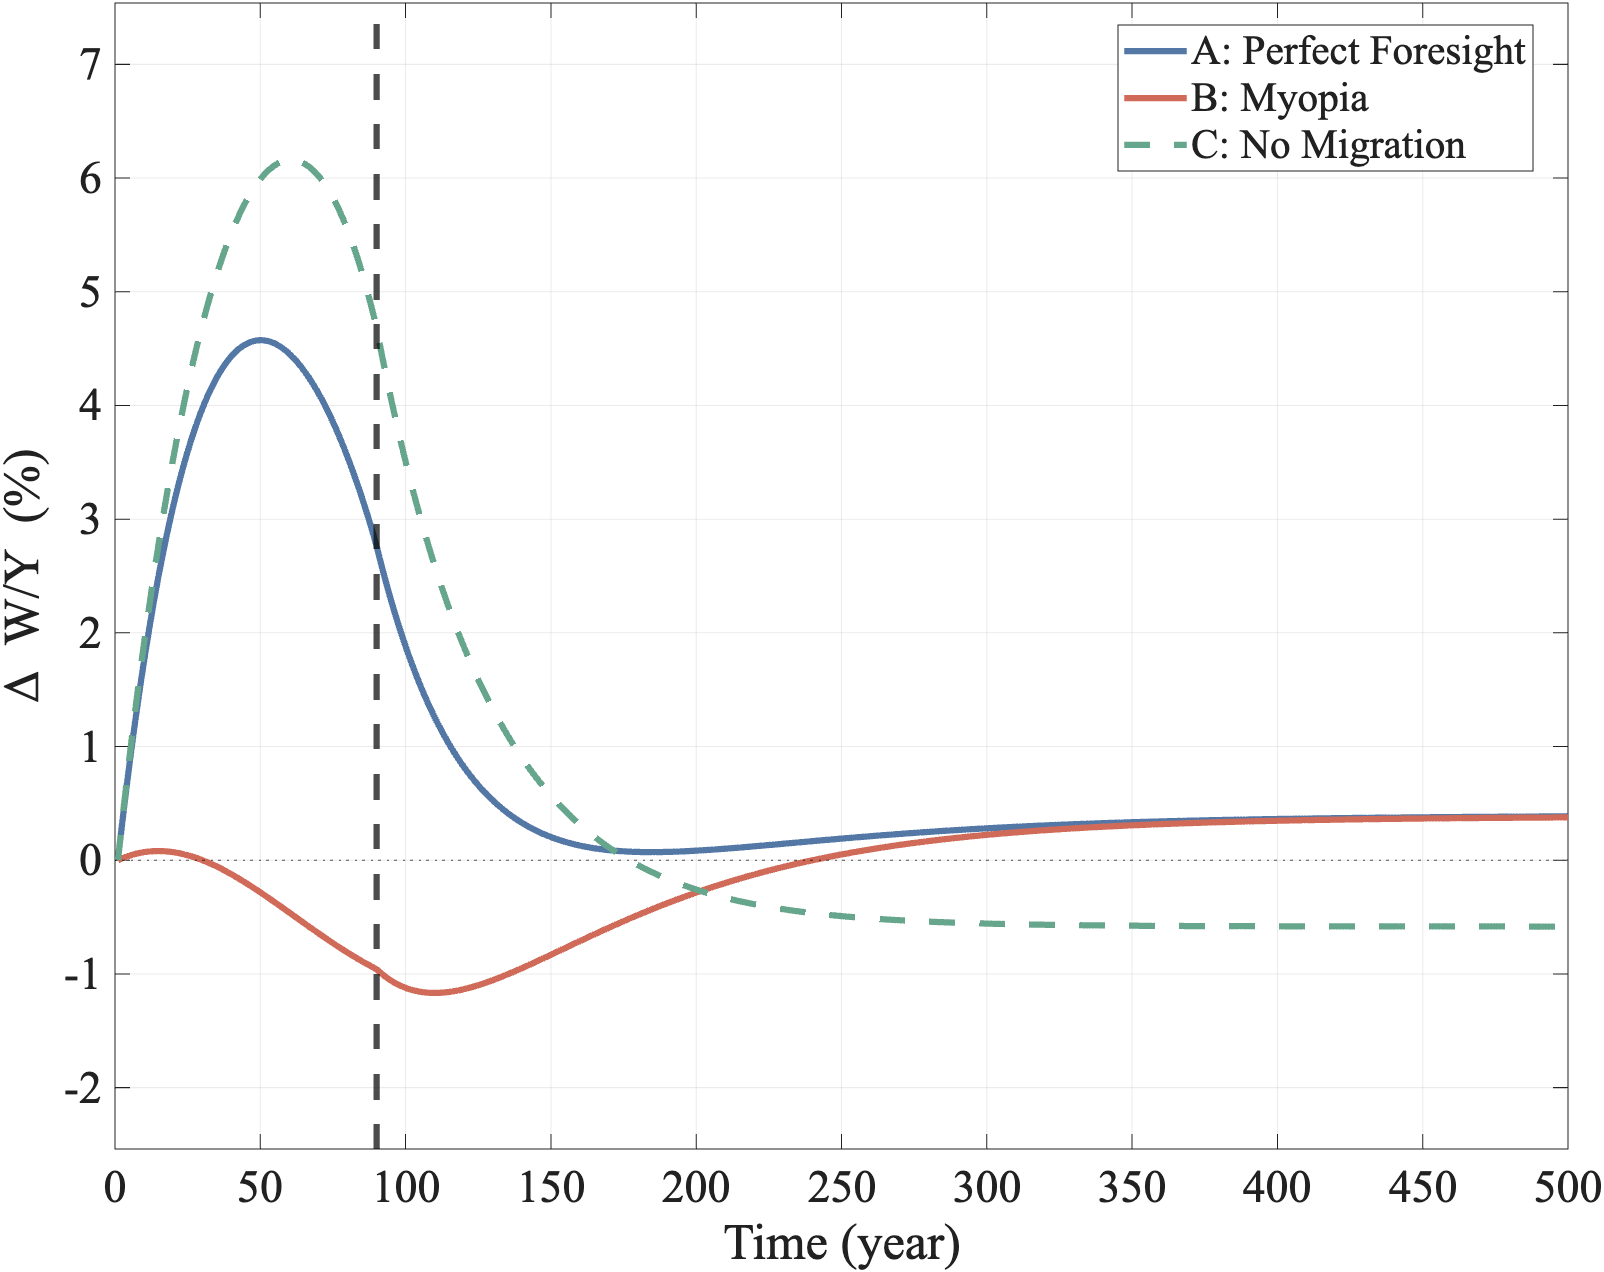
\includegraphics[width=\textwidth]{../Output/big_nu/graph_macro_audit/macro_wy_frictions/macro_wy_frictions_macro_wy_delta_wy_pct.png}
  \end{minipage}\hfill
  \begin{minipage}[t]{0.48\textwidth}
    \centering
    \small{(b) Welfare (CE)}
    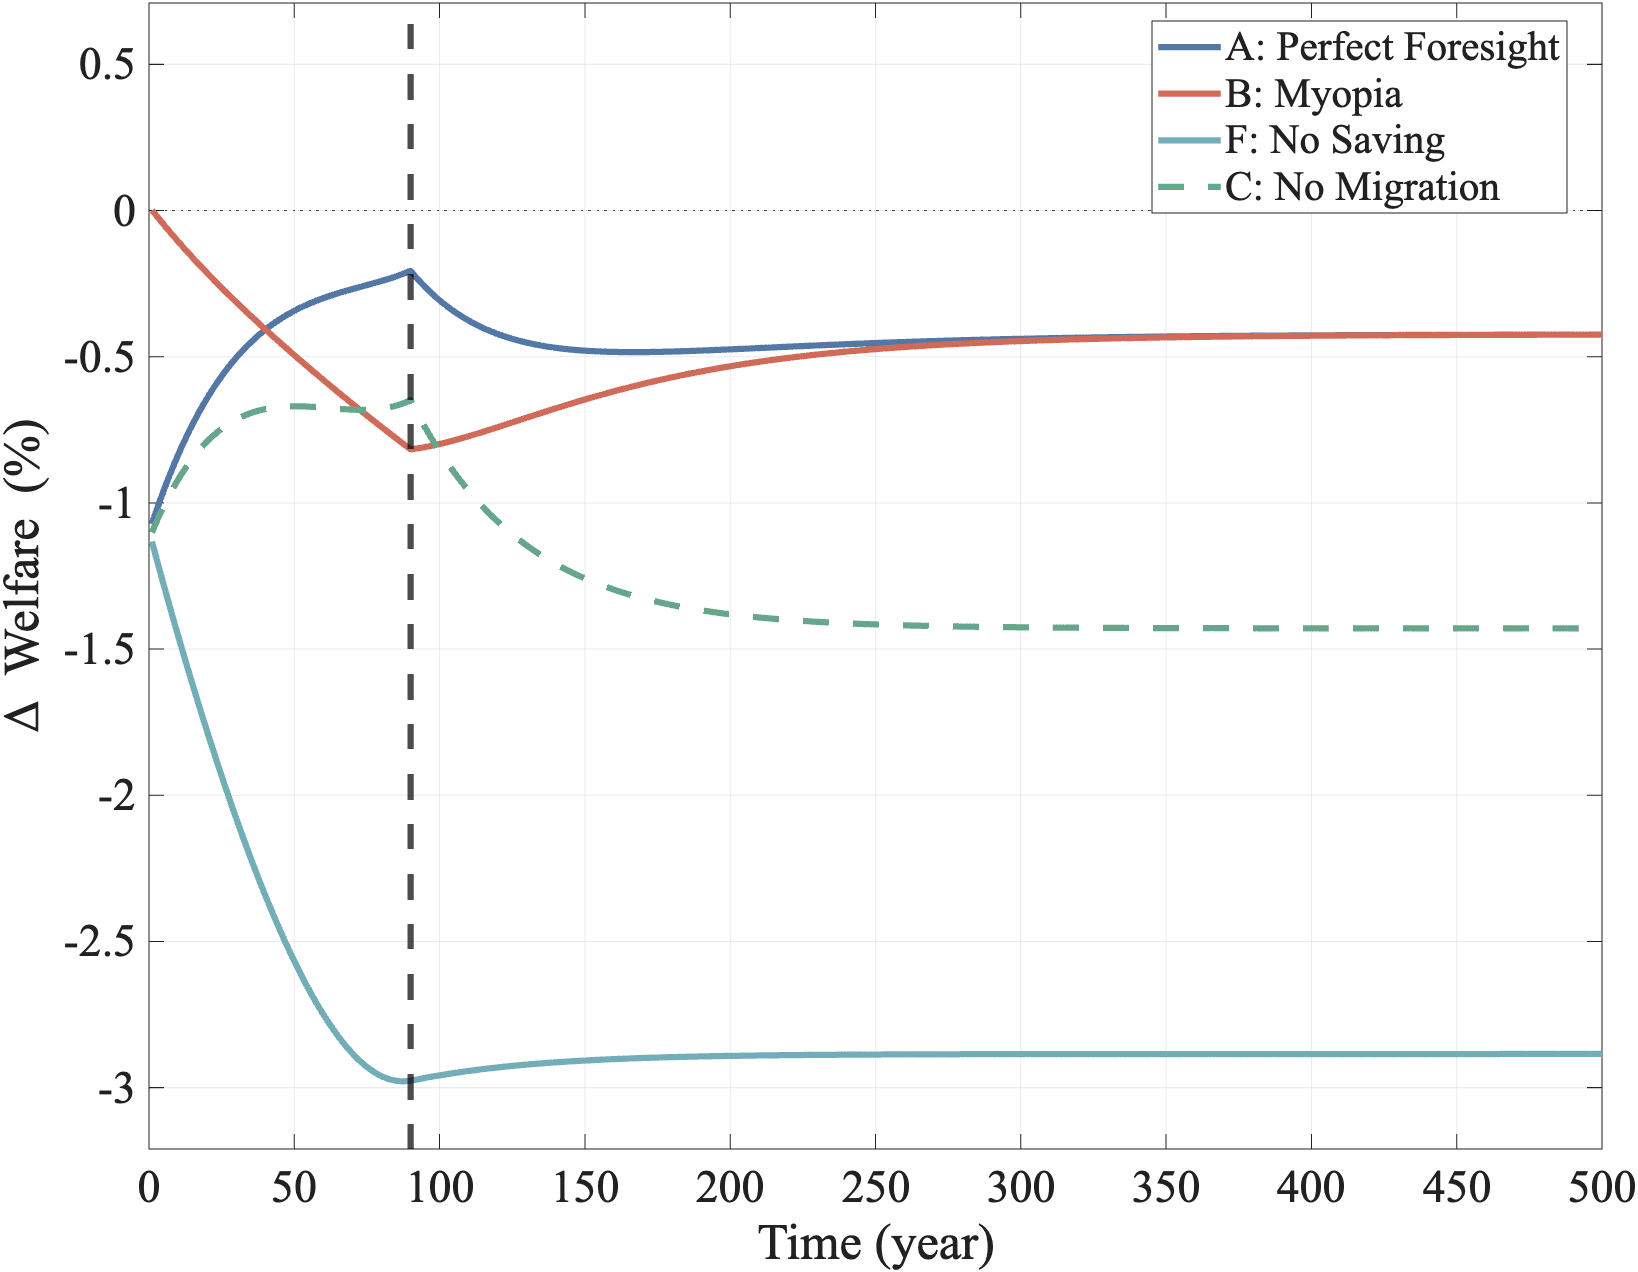
\includegraphics[width=\textwidth]{../Output/big_nu/graph_welfare_audit/welfare_audit_all_scenarios_ce_pct_frictions.png}
  \end{minipage}
  \vspace{0.5em}
  \begin{minipage}{\textwidth}
    \footnotesize{\textbf{Note:} Cross-scenario macro comparison of national aggregate dynamics (for Perfect Foresight, Myopia, No Saving and Autarky scenarios). Panel (a): comparative time series of the wealth-to-earnings ratio $(W/Y)_t = W_t / Y_t$. Panel (b): percentage change in aggregate consumption-equivalent (CE) welfare relative to initial aggregate material consumption.}
  \end{minipage}
  \label{fig:welfare_comp_pc}
\end{figure}

\paragraph{Welfare.} At $t = 1$, so right after the climate shock is realised, the welfare loss is the lowest in the Myopia scenario because agents did not anticipate the coming damages and so wrongly expect the rainy days to not come.\footnote{In the context of climate change, it would perhaps be more accurate to talk about the sunny days...} The other scenarios show a welfare loss of 1\% at $t = 1$, which is the result of the anticipation of future damages and results in precautionary saving. However, as time progresses and climate damages materialise, the Myopia scenario experiences a larger welfare loss compared to the baseline. At $t = 90$, the Myopia scenario shows a welfare loss of 0.8\%, while the baseline scenario shows a welfare loss of 0.2\% thanks to the accumulation of wealth. The No Migration scenario also exhibits a larger welfare loss at $t = 90$ than the baseline, with a decline of 0.65\%, because of the impossibility to move. According to the model, in the short-run it is therefore better to anticipate climate change without moving than to move without anticipation. For the No Saving scenario, the welfare loss is the largest at $t = 90$ with a decline of 3\%, showing that, in the model, saving is a more important mechanism than migration to smooth climate damages. At the terminal steady state, all scenarios show a welfare loss, with the Myopia and baseline scenario stabilising with a decline of 0.5\% and the No Migration scenario shows a welfare loss of 1.5\% three times larger. The No Saving scenario stabilises at -2.8\%. 

\FloatBarrier
\section{Discussion and Conclusion}
\label{sec:discussion}

\paragraph{CARA Utility Function.}
As stated, the model uses a CARA utility function to ensure that the closed-form solution of the model is tractable and has no borrowing constraint. The CARA utility function has the property that the absolute risk aversion is constant and presents no income effect. Economically, this implicitly assumes complete credit markets where agents can finance moving costs. It makes the model blind to spatial poverty traps, wherein low-wealth households are liquidity-constrained and trapped in geographic areas highly exposed to climate damages. By ignoring these frictions, the framework likely overstates the insurance value of migration for the most vulnerable populations.

\paragraph{Partial Equilibrium and Capital Accumulation.}
The framework is a partial equilibrium endowment economy with no production sector. By fixing the interest rate at $r = 0.03$, the model behaves like a small open economy. In a closed general equilibrium setting, the accumulation of wealth during the 2010-2100 period would drive down the equilibrium interest rate and reduce the return on assets. Furthermore, the absence of endogenous production means the model abstracts from direct climate damages to the physical capital stock, which could depress the marginal product of labour and lower wages (assuming complementarity between capital and labour). Overall, the assumption of an exogenous interest rate and lack of capital accumulation facilitates wealth accumulation, and overstates the efficacy of saving as an adaptation mechanism.

\paragraph{Agglomeration and Dispersion Forces.}
The model does not include agglomeration and dispersion forces. For instance, one could expect that the migration of workers from the South to the North would increase congestion in the North, increasing housing costs and reducing amenities, which would reduce the incentive to migrate. The effect of the population change on wage is unclear as more people in the same location might generate positive externalities with economies of scale or create more congestion on the labour market. Overall, it might overstate the ability of workers to adapt to climate change by moving.

\paragraph{Comparison with the Literature.}
The aggregate welfare loss generated by the baseline model is an order of magnitude smaller than estimates found in other spatial climate studies that focused on the US (e.g., \citet{hsiang_estimating_2017}; \citet{bilal_anticipating_nodate}). This difference is driven by the capacity agents have to endogenously adapt through both spatial mobility and precautionary saving. For instance, \citet{hsiang_estimating_2017} is an econometric analysis that mechanically prevents agents from adjusting. \citet{bilal_anticipating_nodate} restrict the adaptive capacity of labour by modelling mobile hand-to-mouth workers and immobile capitalists that can save. Indeed, in my No Saving counterfactual, which restricts agent behaviour to a framework more closely aligned with standard spatial models, the welfare drop scales to an order of magnitude comparable with the existing literature. While the baseline model may underestimate absolute welfare losses due to the omissions discussed above, it serves as a first step in demonstrating that omitting forward-looking anticipation, saving and migration biases the welfare costs of climate change upward.

\paragraph{Policy Implications.} Although this partial-equilibrium endowment framework abstracts from congestion externalities and fiscal instruments, the counterfactual exercises can point to three qualitative lessons for adaptation policy. First, credible long-horizon climate information carries important transitional value: because the baseline and myopic economies converge to the same terminal steady state, the decrease in 2100 welfare losses under perfect foresight comes from early precautionary saving accumulated before damages peak. Public disclosure and dissemination of local climate-risk projections can therefore smooth transitional welfare losses well before physical relocation takes place. Second, mobility support and financial insurance work best when designed jointly rather than in silos. Lowering moving barriers, for instance through relocation assistance or floodplain buyouts, achieves less directional reallocation if displaced workers lack liquidity or portable income insurance to bear the higher earnings volatility of moving to more productive labour markets. Third, the large welfare gap between savers ($-0.5\%$) and hand-to-mouth workers ($-2.8\%$) argues for portable, people-based liquidity support rather than place-based subsidies that tie transfers to damaged origin regions and weaken incentives to relocate.

\paragraph{Conclusion.} This paper develops a dynamic, quantitative spatial model that integrates saving and migration as joint adaptive mechanisms in response to spatially heterogeneous climate change. Extending \citet{dvorkin_geography_2025} to transitional dynamics calibrated to the US economy with damage projections from \citet{hsiang_estimating_2017}, the baseline transition shows that spatial reallocation and anticipatory saving restrict long-run welfare losses to 0.5\%, while reshaping the geography of wealth across states. Even though CARA preferences make individual migration and saving choices independent of current wealth at the consumer's decision stage, counterfactual analyses reveal indirect links operating through continuation values, local income-risk exposure, and spatial option values. Suppressing mobility forces workers to rely on precautionary wealth accumulation, whereas suppressing saving exposes hand-to-mouth migrants to local income variance and diverts them away from high-wage Northern states. Thus, just as savings enable the risk-taking required for directional mobility, spatial mobility shapes the regional distribution of wealth. Finally, in the face of climate change, the relationship between saving and migration is likely even more complex than modelled here; climate-change-induced migration might activate inter-regional financial networks, such as remittances and wealth transfers to support relatives remaining in the origin location.


\appendix
\numberwithin{equation}{section}
\numberwithin{figure}{section}
\numberwithin{table}{section}
% ---------------------------------------------------------
% APPENDIX
% ---------------------------------------------------------
\section{Proofs and Mathematical Derivations}
\label{app:proofs}
\subsection{Aggregation of Individual Consumption and Saving}
Let $\Lambda_{\ell, t}(z^\prime)$ be the density of workers with shock $z^\prime$ in labour market $\ell$ at the end of period time $t$ and $f_\ell$ the pdf of the $\epsilon$. First, the evolution of the population distribution across locations is given by:
\begin{equation}
\Lambda_{\ell,t}(z^\prime) = (1-\delta) \sum_{j=1}^J \int \Lambda_{j,t-1}(z) \mu_{j\ell,t}(z) f_\ell(z^\prime - \rho z) \mathrm{d}z + \sum_{j=1}^J \mu_{j\ell,t}(0) f_\ell(z^\prime) \left( \delta \int \Lambda_{j,t-1}(z) \mathrm{d}z \right)
\end{equation}
where $\delta$ is the exogenous probability of death. The first term captures surviving workers who relocate from any origin $j$ to destination $\ell$ and draw a new persistent shock $z^\prime$, while the second term accounts for newborns (who start with median productivity $z=0$) choosing location $\ell$ and then drawing their first shock $z^\prime$. 

Given the linearity of the optimal decision rules with respect to cash-on-hand, I can aggregate consumption and wealth at the local level. Under a stationary interest rate $r$, the evolution of average consumption $\bar{c}_{\ell,t}(z^\prime)$ and average asset holdings $\bar{a}_{\ell,t+1}(z^\prime)$ for workers with shock $z^\prime$ in labour market $\ell$ are characterised by:
\begin{align}
\bar{c}_{\ell,t}(z^\prime) &= \sum_{j=1}^J \int \frac{\Lambda_{j,t-1}(z)\mu_{j\ell,t}(z)f_\ell(z^\prime - \rho z)}{\Lambda_{\ell,t}(z^\prime)} (1-\delta) \left( \Xi_{\ell,t}(z^\prime) + \frac{r}{1+r} \tilde{y}_{\ell,t} + \frac{r}{1+r} \bar{a}_{j,t}(z) \right) \mathrm{d}z \nonumber \\
&\quad + \sum_{j=1}^J \frac{\mu_{j\ell,t}(0) f_\ell(z^\prime)}{\Lambda_{\ell,t}(z^\prime)} \left( \Xi_{\ell,t}(z^\prime) + \frac{r}{1+r} \tilde{y}_{\ell,t} + \frac{r}{1+r} a_0 \right) \left( \delta \int \Lambda_{j,t-1}(z) \mathrm{d}z \right), \\
\bar{a}_{\ell,t+1}(z^\prime) &= \sum_{j=1}^J \int \frac{\Lambda_{j,t-1}(z)\mu_{j\ell,t}(z)f_\ell(z^\prime - \rho z)}{\Lambda_{\ell,t}(z^\prime)} (1-\delta) \left( \tilde{y}_{\ell,t} + \bar{a}_{j,t}(z) + (1+r)(\tilde{w}_{\ell,t}z^\prime - \Xi_{\ell,t}(z^\prime)) \right) \mathrm{d}z \nonumber \\
&\quad + \sum_{j=1}^J \frac{\mu_{j\ell,t}(0) f_\ell(z^\prime)}{\Lambda_{\ell,t}(z^\prime)} \left( \tilde{y}_{\ell,t} + a_0 + (1+r)(\tilde{w}_{\ell,t}z^\prime - \Xi_{\ell,t}(z^\prime)) \right) \left( \delta \int \Lambda_{j,t-1}(z) \mathrm{d}z \right)
\end{align}
where $a_0$ is the exogenous initial wealth endowed to newborns, and $\bar{a}_{j,t}(z)$ is the average asset holding of workers in labour market $j$ with shock $z$ at the end of period $t-1$. Finally, the aggregate level of wealth and consumption per period $t$ are given by:
\begin{equation}
  \bar{a}_{t+1} = \sum_{\ell=1}^J \int \Lambda_{\ell,t}(z^\prime) \bar{a}_{\ell,t+1}(z^\prime) \mathrm{d}z^\prime, \qquad
  \bar{c}_{t} = \sum_{\ell=1}^J \int \Lambda_{\ell,t}(z^\prime) \bar{c}_{\ell,t}(z^\prime) \mathrm{d}z^\prime.
\end{equation}

\subsection{Derivation of $\Xi$ in the No Saving Scenario}
\label{sec:appendix_no_saving}
When workers consume their full disposable income in every period ($c_{\ell,t} = \tilde{y}_{\ell,t} + \tilde{w}_{\ell,t}z^\prime + \tilde{w}_{\ell,t}\eta^\prime$, where $\tilde{y}_{\ell,t} = (1 - D^w_{\ell,t})w_{\ell,t} - q_{\ell,t}(1+ D^q_{\ell,t})$ and $\tilde{w}_{\ell,t} = (1 - D^w_{\ell,t})w_{\ell,t}$), let $v_{j,t}(z) = -\frac{1}{\gamma} e^{-\gamma \Xi_{j,t}(z)}$ denote the \textit{ex-ante} expected lifetime utility of a worker in location $j$ with productivity $z$. The worker's problem is $v_{j,t}(z) = \mathbb{E}_{\varepsilon} \left[ \max_{\ell} \left\{ \varepsilon_\ell e^{\psi_{j\ell}} U_{\ell,t}(z) \right\} \right]$, where $U_{\ell,t}(z) = \mathbb{E}_{z^\prime, \eta^\prime | z, \ell} \left[ -\frac{1}{\gamma} e^{-\gamma c_{\ell,t} - \tilde{A}_{\ell,t}} + \beta v_{\ell,t+1}(z^\prime) \right]$. Evaluating the intra-period expectation over $\eta^\prime \sim \mathcal{N}(0, \sigma_{\eta, \ell}^2)$ with $F_{\ell,t}(z^\prime) \equiv -\gamma \tilde{y}_{\ell,t} - \gamma \tilde{w}_{\ell,t} z^\prime - \tilde{A}_{\ell,t} + \frac{1}{2}(\gamma \tilde{w}_{\ell,t})^2 \sigma_{\eta,\ell}^2$ yields:
\begin{equation}
U_{\ell,t}(z) = -\frac{1}{\gamma} \mathbb{E}_{z^\prime | z, \ell} \left[ \exp\left(F_{\ell,t}(z^\prime)\right) + \beta \exp\left(-\gamma \Xi_{\ell,t+1}(z^\prime)\right) \right]
\end{equation}

By the properties of the Weibull distribution $\varepsilon_\ell$ (with shape parameter $\nu$ and a normalised scale parameter $\bar{\lambda}$), the expectation of the maximum of these discrete choices yields the closed-form inclusive value:
\begin{equation}
v_{j,t}(z) = -\frac{1}{\gamma} \bar{\lambda} \left[ \sum_{m=1}^J \left( e^{\psi_{jm}} \mathbb{E}_{z^\prime | z, m} \left[ \exp\left(F_{m,t}(z^\prime)\right) + \beta \exp\left(-\gamma \Xi_{m,t+1}(z^\prime)\right) \right] \right)^{-\nu} \right]^{-1/\nu}
\end{equation}
Equating this to $v_{j,t}(z) = -\frac{1}{\gamma} e^{-\gamma \Xi_{j,t}(z)}$, taking the natural logarithm, and rearranging yields Equation~\eqref{eq:Xi_nosaving}.

\section{Algorithm Description}
\label{app:algorithms}
\subsection{Stationary Equilibrium Solves}
Given all estimated and calibrated parameters, the stationary $\Xi^*_\ell(z)$ is the fixed point of operator $\mathcal{T}$ defined by eq.~\eqref{eq:Xi}, initialised at $\Xi^{(0)} = 0$ and iterated until convergence. All numerical expectations are computed using a Rouwenhorst method over the $z$ grid, with a log-sum-exp trick for numerical stability. Warm-starting from the previous $\Xi$ iterate is used inside the calibration exercise and the Myopia scenario to reduce the number of fixed-point iterations per step.

Over the $J \times N_z$ discrete states $k = (\ell, z)$, let $\mathbf{T}$ denote the stationary $(J N_z) \times (J N_z)$ transition matrix from Equation~\eqref{eq:T_sparse}. The stationary population distribution solves $\boldsymbol{\Lambda} \cdot \mathbf{T} = \boldsymbol{\Lambda}$, computed in MATLAB by extracting the left eigenvector associated with the dominant eigenvalue of $1$ via \verb|[eig_vec, ~] = eigs(T_mat', 1, 'lr')|. Letting $S_\ell(z') = \tilde y_\ell + (1+r)\bigl[\tilde w_\ell z' - \Xi_\ell(z')\bigr]$ denote the savings accruing to an agent entering state $(\ell, z')$, the wealth mass vector $\mathbf{A}$ satisfies the Neumann equation:
\begin{equation}
  \mathbf{A} = \boldsymbol{b}_A \cdot (\mathbf{I} - \mathbf{T^{\text{surv}}})^{-1},
  \label{eq:A_inv}
\end{equation}
where $b_A(k) = \Lambda(k) \cdot S(k)$ (not augmented by birth endowments here as $a_0 = 0$). Mean wealth in state $\ell$ is then $\bar a_\ell = \sum_{z} A(\ell, z) / \sum_{z} \Lambda(\ell, z)$.

\subsection{Algorithm for the Spatial Decomposition}
\label{sec:algorithm_spatial_decomp}

Let $s_{\ell,t}(z)$ denote the local savings flow in state $\ell$ with productivity shock $z$ at time $t$, and let $\tilde{T}_t$ denote the time-reversed Markov transition matrix over the state space. Total accumulated wealth is given by the recursive sum $a_t = (I - \tilde{T}_t)^{-1} s_t$.

\paragraph{Step 1: Compute Autarky Counterfactuals.} 
To prevent spatial option values from contaminating the deterministic income channel, I construct first an autarky counterfactual. By imposing infinite moving costs ($\psi_{\ell m} \to \infty$ for $\ell \neq m$), I compute the autarky continuation value $\Xi_{\text{aut}, t}$ and extract the baseline autarky transition matrix $\tilde{T}_{\text{aut}, 0}$ (which is a block-diagonal matrix as people cannot move).

\paragraph{Step 2: Decompose the Saving Rule.}
The change in the local savings flow, $\Delta s_{\ell}(z) = s_{\ell,1}(z) - s_{\ell,0}(z)$, is separated into three fundamental channels:
\begin{align}
    \Delta s_{\text{Dam}} &= \frac{\Delta \tilde{y}_\ell}{1+r} + \Delta \tilde{w}_\ell z - \Delta \mathbb{E}_{z^\prime|z}[\Xi_{\ell,\text{aut}}(z^\prime)] \\
    \Delta s_{\text{Risk}} &= \frac{1}{\gamma} \Delta \log \mathbb{E}_{z^\prime|z}[e^{-\gamma \Xi_{\ell}(z^\prime)}] + \Delta \mathbb{E}_{z^\prime|z}[\Xi_{\ell}(z^\prime)] + \Delta \text{Risk}_{\text{Trans}} \\
    \Delta s_{\text{Spat}} &= \Delta s_{\ell}(z) - \Delta s_{\text{Dam}} - \Delta s_{\text{Risk}}
\end{align}

\paragraph{Step 3: Accumulate Flows into Wealth Stocks.}
The saving rule margins are accumulated using the baseline autarky network $\tilde{T}_{\text{aut}, 0}$:
\begin{align}
    a_{\text{Dam}} &= (I - \tilde{T}_{\text{aut}, 0})^{-1} \Delta s_{\text{Dam}} \\
    a_{\text{Risk}} &= (I - \tilde{T}_{\text{aut}, 0})^{-1} \Delta s_{\text{Risk}}
\end{align}
The \textit{Spatial Option} channel absorbs the network premium:
\begin{equation}
    a_{\text{Spat}} = (I - \tilde{T}_0)^{-1} \Delta s - a_{\text{Dam}} - a_{\text{Risk}}
\end{equation}

\paragraph{Step 4: Isolate Spatial Transition and Compositional Sorting.}
The \textit{Spatial Transition} channel evaluates the network shift at $s_1$:
\begin{equation}
    a_{\text{Trans}} = a_1 - (I - \tilde{T}_0)^{-1} s_1
\end{equation}
The micro-responses are aggregated to the state level $\ell$. To complete the shift-share decomposition on the state-level averages $\bar{a}_{\ell,t}$, I weight the former margins by the baseline demographic shares $\pi_0$, and assign the remaining spatial variation to \textit{Compositional Sorting} of the productivity distribution:
\begin{align}
    \bar{a}_{\ell,1} - \bar{a}_{\ell,0} &= \sum_{z} \pi_0(z|\ell) \left[ a_{\text{Dam}} + a_{\text{Risk}} + a_{\text{Spat}} + a_{\text{Trans}} \right] + \sum_{z} \left( \pi_1(z|\ell) - \pi_0(z|\ell) \right) a_{\ell,1}(z)
\end{align}


\bibliographystyle{plainnat}
\bibliography{../references}

\end{document}